% =====================================================================
%  Ekdant -- MSc thesis draft, compiled from the research vault.
%  Build:  pdflatex thesis.tex   (run three times: TOC, references, convergence)
%  Companion markdown: thesis.md   (same content, vault links intact)
%
%  Every numeric claim in this document is either (a) a config value from
%  09-Code/configs/*.json (documented in 02-Architecture/12_Configuration_Guide.md),
%  (b) a parameter count measured with estimate_model_size or derived in the
%  "Complexity and parameter budget" subsection, (c) a hand-worked number from
%  04-Model-DeepDive/28_Worked_Examples.md, (d) a logged run result (run.md
%  section 6, 09-Code/*.log), or (e) marked [PENDING] because the run has not
%  happened yet.  Nothing is asserted without one of those.
% =====================================================================
\documentclass[11pt,a4paper]{article}

\usepackage[T1]{fontenc}
\usepackage[utf8]{inputenc}
\usepackage[margin=1in]{geometry}
\usepackage{amsmath,amssymb,amsthm}
\usepackage{booktabs,array,longtable}
\usepackage[table,dvipsnames]{xcolor}
\usepackage{graphicx}
\usepackage[font=small,labelfont=bf,skip=4pt]{caption}
\usepackage{tikz}
\usepackage{pgfplots}
\usepackage[hidelinks]{hyperref}

\pgfplotsset{compat=1.18}
\usetikzlibrary{arrows.meta,positioning,calc}
\usepgfplotslibrary{groupplots}

% ---- shared figure styling -------------------------------------------
\definecolor{ekLone}{HTML}{1F4E79}   % L1 / memory
\definecolor{ekTwo}{HTML}{7B3F00}   % L2 / reasoning
\definecolor{ekT}{HTML}{2E6B4F}     % stage T
\definecolor{ekWarn}{HTML}{A11212}
\definecolor{ekInk}{HTML}{22252A}
\definecolor{ekPaper}{HTML}{F4F6F8}
\definecolor{ekEdge}{HTML}{8A94A0}    % neutral structure

% ---- palette used for the shaded table rows --------------------------
\definecolor{ekHeadBG}{HTML}{1F4E79} % table header background
\definecolor{ekRowL}{HTML}{EAF0F6}   % stage L1 rows
\definecolor{ekRowT}{HTML}{E8F1EC}   % stage T rows
\definecolor{ekRow2}{HTML}{F6EFE8}   % stage L2 rows
\definecolor{ekRowW}{HTML}{FBE9E9}   % warning / defect rows

\tikzset{
  ekbox/.style   = {draw=ekEdge, rounded corners=2pt, fill=ekPaper,
                    align=center, inner sep=4pt, font=\footnotesize},
  ekstage/.style = {draw=ekEdge, very thick, rounded corners=3pt, fill=white,
                    align=center, inner sep=5pt, font=\small\bfseries},
  ekflow/.style  = {-{Stealth[length=5pt,width=4pt]}, ekInk, semithick},
  ekloop/.style  = {-{Stealth[length=5pt,width=4pt]}, ekWarn, thick, dashed},
  ektag/.style   = {font=\scriptsize\itshape, text=ekEdge, align=center},
  eklabel/.style = {font=\footnotesize\bfseries, text=ekInk},
}
\tikzset{
  ekstageL/.style = {ekstage, draw=ekLone, fill=ekLone!6},
  ekstageT/.style = {ekstage, draw=ekT,   fill=ekT!6},
  ekstage2/.style = {ekstage, draw=ekTwo, fill=ekTwo!6},
}

% ---- notation macros -------------------------------------------------
\newcommand{\sdim}{d_{\text{state}}}
\newcommand{\Hdim}{H}
\newcommand{\Bdim}{B}
\newcommand{\Tdim}{T}
\newcommand{\Vdim}{V}
\newcommand{\Ldim}{L}
\newcommand{\Kdim}{K}
\newcommand{\Rdim}{R}
\newcommand{\Sdim}{S}
\newcommand{\etadim}{\eta}
\newcommand{\rhodim}{\rho}
\newcommand{\lam}{\lambda}
\newcommand{\Atr}{\bar{A}}
\newcommand{\Btr}{\bar{B}}
\newcommand{\Cdim}{\bar{C}}
\newcommand{\Rt}{\mathrm{RMSNorm}}
\newcommand{\sm}{softmax}
\newcommand{\Var}{\mathrm{Var}}
\newcommand{\E}{\mathbb{E}}
\newcommand{\hd}{\mathrm{head}}

% ---- theorem environments -------------------------------------------
\theoremstyle{plain}
\newtheorem{proposition}{Proposition}
\newtheorem{corollary}[proposition]{Corollary}
\theoremstyle{definition}
\newtheorem{definition}{Definition}
\theoremstyle{remark}
\newtheorem{remark}{Remark}

% Document metadata lives in \hypersetup below; the title page is built by hand,
% so \title/\author/\date are deliberately not declared.

\hypersetup{
  pdftitle={Ekdant: A Parallel Sandbox with Anchored Gated Descent for Medical Multiple-Choice Reasoning},
  pdfauthor={Harshil Gorasiya},
  pdfsubject={MSc thesis --- Hochschule Heilbronn},
  pdfkeywords={windowed transformer, sandbox, anchored gated descent,
               medical question answering, MedMCQA, MedQA, readout invariance},
}

\begin{document}

% ---- title page ------------------------------------------------------
\begin{titlepage}
\thispagestyle{empty}
\centering
\vspace*{3.2cm}

{\color{ekLone}\rule{\textwidth}{1.4pt}}\\[0.5cm]
{\Huge\bfseries Ekdant\par}
\vspace{0.7cm}
{\large A Parallel Sandbox with Anchored Gated Descent\\[0.25cm]
for Medical Multiple-Choice Reasoning\par}
\vspace{0.6cm}
{\color{ekLone}\rule{\textwidth}{1.4pt}}

\vspace{2.6cm}

\begin{minipage}{0.82\textwidth}
\centering\small
A windowed dense Transformer (T) topped by a parallel debate sandbox with
anchored gated descent (L2), trained from scratch on MedMCQA and MedQA. The
selective state-space store (L1) is specified in this document and left as
future work.
\end{minipage}

\vfill

{\Large\bfseries Harshil Gorasiya\par}
\vspace{0.7cm}

{\large MSc Thesis\par}
\vspace{0.25cm}
{\normalsize Hochschule Heilbronn\par}
\vspace{0.6cm}

\begin{minipage}{0.72\textwidth}
\centering\small
\begin{tabular}{@{}r@{\quad}l@{}}
Supervisor:      & \textbf{[Supervisor 1]} \\
Co-supervisor:   & \textbf{[Supervisor 2]} \\
\end{tabular}
\end{minipage}

\vspace{0.9cm}

{\small Compiled draft generated from the research vault --- \today\par}

\vspace{0.8cm}
{\small\itshape Every numeric claim is either a configuration value, a measured parameter
count, a hand-worked derivation, a logged run result, or marked
\texttt{[PENDING]}.\par}
\end{titlepage}

% ---- abstract (roman numerals) --------------------------------------
\pagenumbering{roman}
\pagestyle{plain}

\begin{abstract}
\noindent
Transformer decoders scale quadratically in context length and their
key--value (KV) cache grows without bound, so a model intended to reason over
long inputs pays the most exactly where it should be strongest. Separately, a
monolithic stack cannot say which component is responsible for a gain, and
self-reported confidence is uncalibrated: agreement between reasoning paths is
routinely mistaken for certainty even though agreement is trivially maximized
by collapsing all paths onto one answer.

\noindent
Ekdant is a three-stage design that makes each of these addressable and,
crucially, makes its own design falsifiable. Stage L1 is a selective
state-space layer with three L1 state stores (content, control, sandbox), giving
linear-time training and a fixed-size inference state independent of sequence
length; it is \emph{specified and analysed here but not implemented}. The
built and evaluated model consists of the other two stages. Stage T is a plain
dense Transformer stack---windowed grouped-query attention with rotary
positions and SwiGLU feed-forward blocks---whose only job is to bound the KV
cache and provide local exact retrieval. Stage L2 is a sandbox: $K$ parallel
trajectories that cross-read for $R$ debate rounds and then perform $S$ steps
of \emph{anchored gated descent} on an explicit energy before a single dense
head produces logits. The sandbox is the debate layer; the L1 store is SSM
memory, and the write-back that would couple them awaits L1.

\noindent
Two training signals are used, and the second one is the subject of a
correction. We originally specified an agreement penalty between trajectories;
we proved it is minimized by the very collapse it is meant to detect, and
replaced it with a dimensionless collapse \emph{floor} that is exactly zero
while the hypotheses remain diverse. We also proved that the natural energy
update---descending toward the running mean of the trajectories---is
\emph{readout-invariant} and therefore cannot change the model's output at all,
and replaced it with an externally anchored, per-trajectory gated step that
provably decreases each trajectory's energy and does move the readout. Both
defects, their proofs, and their numerical consequences are reported rather
than removed. A first, from-scratch evaluation (an architecture-matched A/B
at 50.09M versus 43.53M parameters on MedMCQA and MedQA) learned only the
answer-letter prior: every score sat at the rate of always choosing the most
common letter, so it could not test L2. The evaluated configuration therefore
places L2 on a pretrained SmolLM2-135M backbone as a zero-initialised gated
residual, scaled to the same share of the model (19.59M of 154.11M
parameters), and compares two arms that start identical: the backbone alone
and the backbone with L2. Both are trained on PubMedQA (question and abstract to conclusion), fine-tuned
on half of MedQuAD and benchmarked once on the other half, split by question,
using reference-answer perplexity with a paired-bootstrap confidence interval
as the primary measure. Every falsifiable claim in the supporting vault
is backed by one of 66 locally stored papers or by an explicit hand
derivation, and an explicit prior-art audit states which claims are \emph{not}
novel---including a compute-matched study in our own library that reports no
reliable gain from the closest published analogue of stage L2.
\end{abstract}

\clearpage

% ---- table of contents, own page -------------------------------------
\tableofcontents

\clearpage

% ---- body, arabic numerals ------------------------------------------
\pagenumbering{arabic}

% =====================================================================
\section{Introduction}
% =====================================================================

\subsection{The problem}

\noindent
Three failure modes motivate this work. They are stated separately because
each has a different, non-interchangeable fix.

\paragraph{P1: Memory grows with the sequence.}
Self-attention compares every position with every other position, giving
quadratic training cost in sequence length, and inference requires a KV cache
that grows linearly in context length. A model meant to reason over long
inputs---source codebases, medical records, papers with cross-references---is
most expensive precisely on its intended inputs.

\paragraph{P2: A monolithic stack cannot be audited.}
When every component lives in one homogeneous stack, a benchmark gain cannot
be attributed to a specific mechanism. Adding capacity and adding a mechanism
are indistinguishable from the outside, so the resulting claim is
unfalsifiable.

\paragraph{P3: Agreement is not confidence.}
A single autoregressive pass emits one answer with one probability
distribution. When it is wrong, nothing records which step went wrong. A
common remedy is to sample several reasoning paths and treat their agreement
as a confidence signal. This remedy has a degenerate optimum that is rarely
discussed: if all paths are made to agree, agreement is perfect and the model
is confidently wrong. The fix is not to avoid agreement but to make the
mechanism that \emph{produces} agreement incapable of benefiting from
collapse.

\subsection{Contributions}

\begin{enumerate}
  \item \textbf{A minimal three-stage split} (L1 selective SSM storage $\to$
        T dense local attention $\to$ L2 parallel sandbox) in which each
        stage exists to solve one of P1--P3, and each can be ablated
        independently. The T and L2 stages are implemented and tested; L1 is
        specified only, so P1 is addressed by design and not by experiment.
  \item \textbf{Anchored gated descent (AGD)} for stage L2, introduced to
        replace a peer-mean energy update that we prove is
        readout-invariant. AGD admits a monotone-energy proof
        (Proposition~\ref{prop:agd-monotone}) and is verified numerically.
  \item \textbf{A dimensionless collapse floor} replacing a degenerate
        agreement penalty, with a proof that the original term is minimized
        at zero spread (Proposition~\ref{prop:agreement-degenerate}) and a
        proof that the replacement is non-degenerate
        (Proposition~\ref{prop:floor-nondegenerate}).
  \item \textbf{An audit that reports its own defects.} Four defects were
        found by internal review, each with a proof, a numerical
        demonstration, and a retained ablation that exhibits the broken
        behavior (Section~\ref{sec:audit}).
  \item \textbf{A self-limiting novelty claim.} A prior-art audit over 30
        sandbox papers and 36 background papers concludes that \emph{every
        ingredient} of stage L2 has precedent, that only the combination plus
        the memory write-back is unclaimed, and---importantly---that the
        closest compute-matched published study reports \emph{no reliable
        gain} for its own version of this mechanism
        (Section~\ref{sec:counter-evidence}).
  \item \textbf{A clean test of L2 on a pretrained backbone.} L2 enters
        as a zero-initialised gated residual, so both arms start as the same
        pretrained model and any later difference is caused by training L2
        (Section~\ref{sec:v2}).
  \item \textbf{A falsifiability apparatus.} 66 locally stored papers, a
        claim-to-evidence index, hand-worked numerical examples requiring only
        a calculator, and a cost-matched evaluation protocol that fixes the
        comparison before any run is performed.
\end{enumerate}

\subsection{Research questions}

\begin{description}
  \item[RQ1 (memory; future work)] Does a fixed-size selective SSM state
    replace the KV cache while preserving long-range recall, and what does it
    cost in exact retrieval? This requires L1, which is not implemented, so
    RQ1 is not tested in this thesis; the protocol is kept in
    Section~\ref{sec:rq1} so the follow-up is pre-specified.
  \item[RQ2 (reasoning)] On generative medical question answering, does
    adding the $K$-trajectory sandbox to a pretrained backbone lower the
    perplexity of held-out reference answers more than further training of
    the backbone alone? The comparison is architecture-matched, not
    parameter-matched: the sandbox arm carries $+19.59$M parameters and extra
    compute (Section~\ref{sec:v2}).
  \item[RQ3 (honesty)] Is trajectory agreement calibrated against per-example
    accuracy, and can collapse be detected early by a monitored statistic
    rather than discovered post hoc?
\end{description}

\subsection{Non-goals and scope}

\noindent
Ekdant is a text-only model. The evaluated configuration adds stage L2 to a
pretrained 135M-parameter backbone (SmolLM2-135M) and trains it on two medical
question-answering datasets (PubMedQA and MedQuAD); a from-scratch 50M pilot on
MedMCQA and MedQA is reported as the motivation. It is not a general-purpose
language model. It is
not a tool-using agent (the ReAct line of work \cite{yao2022react} is cited to
draw this boundary explicitly), not multimodal, and not a mixture-of-experts
model. At this scale, mixture-of-experts and sparse/dense hybrids add routing
machinery without the capacity to exploit it; stage L2 spends the same
parameters on hypothesis diversity instead. Every component is implemented in
plain PyTorch with no external CUDA kernels (the pretrained backbone is loaded
through the \texttt{transformers} library), which keeps the thesis
reproducible and auditable at the cost of raw speed
(Section~\ref{sec:limitations}).

\subsection{Notation}

\begin{center}
\small
\begin{tabular}{@{}>{\raggedright\arraybackslash}p{0.16\linewidth}>{\raggedright\arraybackslash}p{0.76\linewidth}@{}}
\toprule
\rowcolor{ekHeadBG}\color{white}\textbf{Symbol} & \color{white}\textbf{Meaning} \\
\midrule
$B$ & batch size \\
$T$ & sequence length (maximum 2048; no training example is truncated) \\
$V$ & vocabulary size (32{,}768 allocated; 26{,}766 learned by the tokenizer) \\
$H$ & model width (512 as built; design sizes XS / S / M were 256 / 320 / 512) \\
$d$ & per-store state dimension $\sdim$ (L1, design only: 96 / 128 / 256) \\
$N$ & number of L1 blocks (design only: 2 / 4 / 4); the built model has $N_{\mathrm{T}}{=}12$ T blocks \\
$K$ & number of sandbox trajectories (4) \\
$R$ & number of debate rounds (2) \\
$S$ & number of descent steps (8) \\
$W$ & attention window (512) \\
$\rhodim$ & \emph{spread ratio}, the dimensionless collapse monitor \\
$\rhodim_{\min}$ & collapse floor threshold (0.05) \\
\bottomrule
\end{tabular}
\end{center}

\noindent
One naming caution, because two separate stages share a word. Stage~L2 is
\emph{the sandbox}: the parallel debate layer. $S^{\mathrm{sandbox}}$ is one of
the three state stores \emph{inside} stage~L1---a fixed-size SSM memory, not a
layer. L1 and L2 are distinct stages, and their only coupling is the M3
write-back (\S\ref{sec:m3}), which writes L2's consensus into the
$S^{\mathrm{sandbox}}$ store. Elsewhere in this document ``sandbox'' alone
always means the L2 layer, and the store is always written with its
$S^{\,\cdot}$ decoration or as ``the L1 sandbox store''.

% =====================================================================
\section{Background}
% =====================================================================

\subsection{Selective state-space models}

\noindent
A classical linear state-space model maps an input signal through a latent
state,
\begin{equation}
  \dot{x}(t) = A x(t) + B u(t), \qquad y(t) = C x(t),
  \label{eq:ssm-continuous}
\end{equation}
with no skip term ($D = 0$). Such a model is inherently recurrent and has
constant memory, but for many years was empirically weak at long-range
recall. Four results turned it into a competitive neural memory, and stage L1
follows them in order.

\paragraph{Structured parameterization and principled initialization.}
HiPPO theory \cite{gu2020hippo} derives the optimal online projection of
history onto polynomial bases, and S4 \cite{gu2021s4} builds a deep sequence
model on that basis which handles 16K-length tasks.

\paragraph{Diagonal and simplified variants retain the power.}
Diagonal state matrices \cite{gu2022s4d}, multi-input multi-output
formulations with a single scan \cite{gupta2022dss}, and S5
\cite{smith2022s5} match S4 with simpler implementations and parallelizable
recurrences.

\paragraph{Input-dependent selection.}
Making the dynamics---the step size and the input/output projections---functions
of the input allows the state to forget selectively. This is the step that
closes copying and induction-style retrieval gaps and extrapolates far beyond
training length \cite{gu2023mamba}. It is the core mechanism of stage L1. The
duality framework unifying this with attention, and the multi-head
state-space design that makes the projections cheap, are in
\cite{dao2024mamba2}.

\paragraph{Hybridization as the honest fallback.}
Pure SSMs trail attention on exact associative recall, and hybrid models win
there \cite{lieber2024jamba}. We treat this as a bound on our claims rather
than a problem to engineer away: stage T exists partly to reintroduce local
exact retrieval.

\noindent
The wider family was surveyed and positioned rather than ignored: long
convolutions \cite{poli2023hyena}, gated SSMs \cite{fu2022h3}, retention
\cite{sun2023retnet}, modern RNNs \cite{peng2023rwkv,de2024griffin,beck2024xlstm},
byte-level selectivity \cite{wang2024mambabyte}, multidimensional states
\cite{nguyen2022s4nd}, and liquid time-constants \cite{hasani2022liquid}. The
efficiency bar we hold ourselves to is IO-aware exact attention
\cite{dao2022flashattn}, and the standard benchmark framing for this family is
the Long Range Arena \cite{tay2020lra}.

\subsection{The dense Transformer block}

\noindent
Stage T is the standard pre-norm decoder block of Vaswani et al.~\cite{vaswani2017},
with four well-understood modifications, each chosen for a specific reason.

\paragraph{RMSNorm and pre-norm.}
Root-mean-square (RMS) normalization \cite{zhang2019rmsnorm} removes the
mean-centering step of LayerNorm, and placing the norm before the residual
\cite{xiong2020prenorm} stabilizes deep stacks without a warmup-schedule hack.
Both are used in every block.

\paragraph{Rotary position embeddings.}
Positions are injected by rotating query and key pairs by an angle that
depends only on relative distance \cite{su2021rope}. Because the rotation
composes, a position $m$ apart is represented by a rotation of $m\theta$,
which is what makes extrapolation and window-relativity behave. No learned
absolute position table is used, so there is no table to grow with context.
For the same reason no RoPE frequency rescaling is used. The rotary base is
$10^5$ and sequences are at most $2048$ tokens (the longest training example
has 857), so plain RoPE never extrapolates and the extension factors of YaRN
\cite{peng2023yarn} would be tuned constants with no failure to repair.
Context extension is not implemented; it matters only for longer-context runs.

\paragraph{Grouped-query attention.}
Multi-query attention \cite{shazeer2019mqa} shares a single key/value head
across all query heads; grouped-query attention \cite{ainslie2023gqa}
interpolates between that and full multi-head attention by using a small
group. We use 8 query heads and 2 key/value heads. The KV cache therefore
costs $2 \times \Tdim \times \hd$ entries per layer instead of
$8 \times \Tdim \times \hd$, a $4\times$ reduction in the dominant cache term
at unchanged attention quality in the cited results.

\paragraph{SwiGLU feed-forward.}
The feed-forward block uses a gated linear unit with a SiLU activation
\cite{shazeer2020glu}: two parallel projections into an intermediate space,
elementwise product, then projection out. This parameterization consistently
outperforms a plain ReLU MLP at fixed parameter count.

\paragraph{Windowed attention.}
Attention is restricted to a window of $W = 512$ preceding tokens
\cite{jiang2023mistral}. This is what actually bounds the cache: cost per
layer is $O(TW)$ rather than $O(T^2)$, and memory is $O(W)$ per sequence
rather than $O(T)$. The exact bound holds when the softmax is computed exactly;
an IO-aware fused kernel reduces memory traffic without changing the math
\cite{dao2023fa2}, which is why we specify the mathematics rather than a
particular attention kernel. Sliding-window attention is also the natural
partner of recurrent state, since the two cover complementary distance ranges.

\subsection{Multi-hypothesis reasoning and consensus}

\noindent
Reasoning traces improve prediction \cite{wei2022cot}; sampling several and
voting beats one greedy path at matched budget \cite{wang2022sc}; letting
paths read and revise each other helps further
\cite{du2023debate,liang2023divergent}; keeping live alternatives with
aggregation beats resampling only at the end \cite{yao2023tot,besta2024got};
and decomposing hard problems into easier ones needs no planner
\cite{zhou2022l2m}. Reflection loops can be folded into latent refinement
\cite{shinn2023reflexion,madaan2023selfrefine}, and per-step supervision beats
outcome-only supervision for reranking \cite{lightman2023verify,uesato2022processfb},
with self-generated rationales usable as targets
\cite{huang2022selfimprove,zelikman2022star}. Multi-agent debate has also been
cast explicitly as a evaluation of communication rather than of a single
reasoner \cite{chan2023chateval}, which is the same move stage L2 makes: the
object of study is whether independently generated trajectories inform each
other, not whether any one of them is correct.

\noindent
Two constraints from this literature shape the evaluation rather than the
architecture. First, cost honesty is load-bearing: debate systems frequently
\emph{tie} voting ensembles at equal budget and are sensitive to tuning
\cite{smit2024mad}, so every result in Section~\ref{sec:eval} is reported
cost-matched with tokens and FLOPs stated, never against greedy decoding
alone. Second, calibration is the deciding measurement
\cite{guo2017calibration}: agreement is only a useful confidence signal if it
predicts per-example accuracy, which is exactly RQ3.

\subsection{Energy-based refinement}

\noindent
Refinement can be framed as descending an energy to a fixed point rather than
as a stack of residual layers. The Energy Transformer iterates a block to
reduce a global energy \cite{energytransformer2023}, and recent work performs
a fixed number of gradient steps on a \emph{parameterized} energy as the
forward pass \cite{nrgpt2025}. Latent-thought calibration pushes intermediate
representations toward low-energy, high-consistency regions
\cite{energycal2025}. This is the direct ancestor of stage L2's descent, and
Section~\ref{sec:defect1} records a failure mode we hit when implementing it
naively.

\subsection{Collapse in reinforcement learning, and why agreement penalties are degenerate}
\label{sec:rl-collapse}

\noindent
This subsection exists because it determines a design decision in
Section~\ref{sec:loss}. In maximum-entropy reinforcement learning, the
standard regularizer trades reward against divergence from the reference
policy, and there is a large literature documenting that this trade
\emph{encourages} mode collapse: the KL term's pressure toward the reference
can be satisfied by reducing the number of distinct solutions rather than by
improving any of them \cite{li2026klcollapse}, and entropy collapse is
documented in RL-with-verifiable-rewards pipelines \cite{acl2026entropy}.

\noindent
The mechanism transfers directly to our setting. If a training term rewards
agreement between trajectories, the cheapest way to reduce it is to make all
trajectories identical---which destroys the diversity the term was introduced
to exploit. This is not a tuning problem; it is an optimization direction
pointing at the wrong optimum. Proposition~\ref{prop:agreement-degenerate}
in Section~\ref{sec:defect2} states and proves the point for our exact loss,
and Section~\ref{sec:loss} gives the replacement.

\subsection{What is claimed as novel, and what is not}

\noindent
The prior-art audit (\texttt{04-Model-DeepDive/\_Prior\_Art\_and\_Novelty\_Check.md})
reached an uncomfortable but clear conclusion: every ingredient of stage L2 has
published precedent.

\begin{center}
\small
\begin{tabular}{@{}>{\raggedright\arraybackslash}p{0.26\linewidth}>{\raggedright\arraybackslash}p{0.66\linewidth}@{}}
\toprule
\rowcolor{ekHeadBG}\color{white}\textbf{Ingredient} & \color{white}\textbf{Precedent} \\
\midrule
Parallel hypothesis streams in one model & Multi-Stream Transformers \cite{burtsev2021multistream} \\
Streams that read and revise each other & Talking-Heads Attention \cite{shazeer2020talkingheads} \\
Function-separated streams at small scale & Dual-Stream Transformer \cite{kerce2026dualstream} \\
Iterative latent refinement, weighted readout & Autoregressive TRM \cite{rauba2026trm}; Coconut; original TRM \cite{jolicoeur2025trm} \\
Descending an energy to a fixed point & Energy Transformer \cite{energytransformer2023}; NRGPT \cite{nrgpt2025} \\
Layered proposal/aggregation & Mixture-of-Agents \cite{wang2025moa} \\
Divergent initialization for multiple paths & Divergent Debate \cite{liang2023divergent} \\
Rationale-aware early stopping & RASC \cite{wan2025rasc} \\
\bottomrule
\end{tabular}
\end{center}

\noindent
Accordingly the novelty claim is restricted to the \emph{combination} and to
one specific mechanism: multi-trajectory tensor-level debate placed after a
dense backbone, whose consensus is written back into an SSM state store. No
single component is claimed as new. Section~\ref{sec:counter-evidence}
discusses the strongest published evidence against even this.

% =====================================================================
\section{Method}
\label{sec:method}

\subsection{Overview}

\noindent
The full design is a single chain with no external calls:
\begin{equation}
  \begin{split}
  \texttt{input\_ids} &\;\to\; \text{L1 (SSM storage)}
    \;\to\; \text{T (dense local attention)}\\
  &\;\to\; \text{L2 (sandbox)} \;\to\; \text{output head}.
  \end{split}
  \label{eq:pipeline}
\end{equation}
Shapes: L1 and T each map $[B,T,H] \to [B,T,H]$; L2 maps $[B,T,H] \to [B,T,H]$
through $K$ trajectories of the same shape. No hidden states grow with $T$ at
inference time.

\paragraph{What is built.}
The implementation evaluated in this thesis omits L1 and the M3 write-back:
\begin{equation}
  \texttt{input\_ids} \;\to\; \text{embed} \;\to\; \text{T (windowed dense)}
  \;\to\; \text{L2 (sandbox)} \;\to\; \text{tied output head},
  \label{eq:built}
\end{equation}
with a baseline arm that deletes L2 and nothing else. Stage T still bounds the
KV cache at the window $W$; the $O(1)$-in-$T$ state claims in this section
hold only for the full design with L1. Everything about L1 below is a
specification, not a result.

Figure~\ref{fig:pipeline} draws that chain, annotates what is bounded and what
is not, and shows the one non-obvious edge: the M3 write-back that returns
L2's consensus into L1's third state store. That dashed edge is what makes
this a memory/reasoning loop rather than a three-block sandwich.

Every diagram in this document uses one fixed colour code, given once here and
never varied: \emph{blue} is L1 and therefore storage, \emph{green} is stage T
and therefore local dense compute, \emph{orange} is L2 and therefore
reasoning, \emph{red dashed} marks the feedback path, and \emph{grey} is a
neutral tensor or projection that belongs to no stage. The same code colours the
row groups of the tables, so a reader can tell at a glance which stage a number
belongs to. Figure~\ref{fig:colourkey} is the key.

\begin{figure}[htbp]
\centering
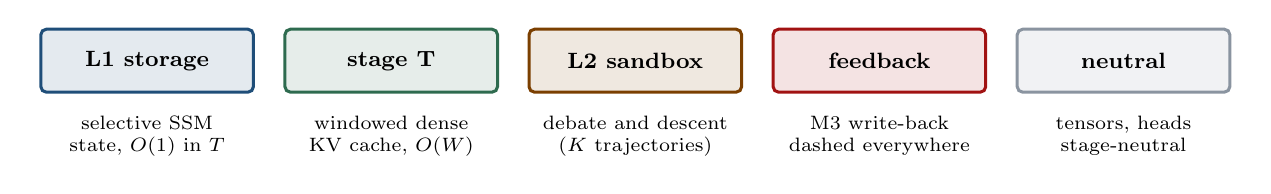
\begin{tikzpicture}
  \node[draw=ekLone, fill=ekLone!12, line width=1.1pt, rounded corners=2pt,
        minimum width=27mm, minimum height=8mm, align=center,
        font=\footnotesize\bfseries] (k1) at (0,0) {L1 storage};
  \node[below=1.6mm of k1, font=\scriptsize, align=center, text width=28mm]
    {selective SSM\\state, $O(1)$ in $T$};

  \node[draw=ekT, fill=ekT!12, line width=1.1pt, rounded corners=2pt,
        minimum width=27mm, minimum height=8mm, align=center,
        font=\footnotesize\bfseries] (k2) at (31mm,0) {stage T};
  \node[below=1.6mm of k2, font=\scriptsize, align=center, text width=28mm]
    {windowed dense\\KV cache, $O(W)$};

  \node[draw=ekTwo, fill=ekTwo!12, line width=1.1pt, rounded corners=2pt,
        minimum width=27mm, minimum height=8mm, align=center,
        font=\footnotesize\bfseries] (k3) at (62mm,0) {L2 sandbox};
  \node[below=1.6mm of k3, font=\scriptsize, align=center, text width=28mm]
    {debate and descent\\($K$ trajectories)};

  \node[draw=ekWarn, fill=ekWarn!12, line width=1.1pt, rounded corners=2pt,
        minimum width=27mm, minimum height=8mm, align=center,
        font=\footnotesize\bfseries] (k4) at (93mm,0) {feedback};
  \node[below=1.6mm of k4, font=\scriptsize, align=center, text width=28mm]
    {M3 write-back\\dashed everywhere};

  \node[draw=ekEdge, fill=ekEdge!12, line width=1.1pt, rounded corners=2pt,
        minimum width=27mm, minimum height=8mm, align=center,
        font=\footnotesize\bfseries] (k5) at (124mm,0) {neutral};
  \node[below=1.6mm of k5, font=\scriptsize, align=center, text width=28mm]
    {tensors, heads\\stage-neutral};
\end{tikzpicture}
\caption{The colour code used in every figure and in the row groups of every
table. Colour is redundant with position and with the labels themselves---it is
a reading aid, never the sole carrier of meaning---but it is applied
consistently from this point on.}
\label{fig:colourkey}
\end{figure}

\begin{figure}[htbp]
\centering
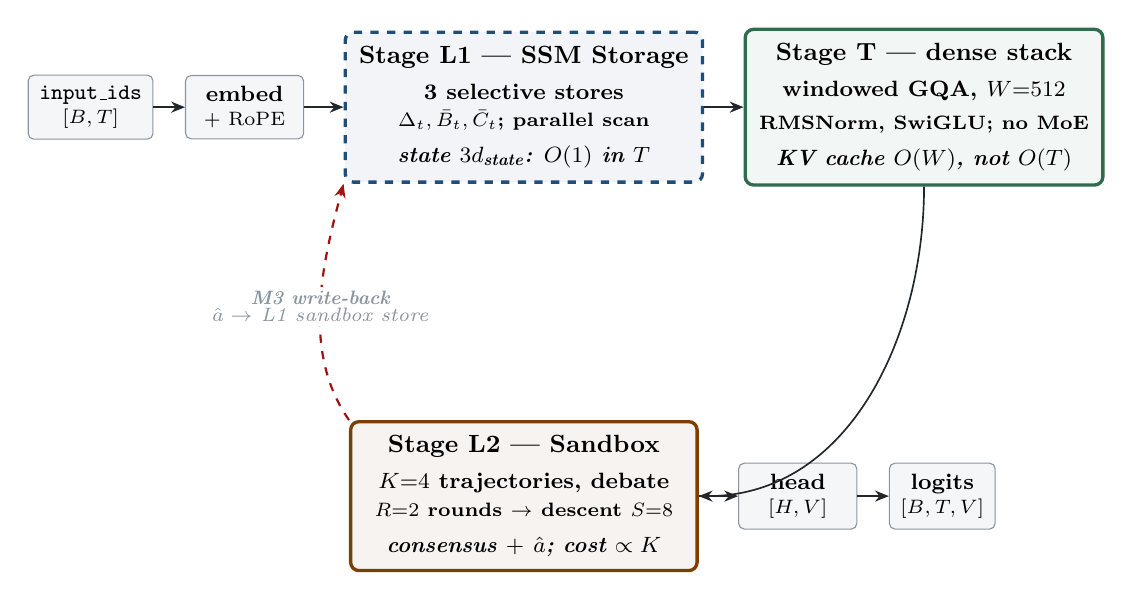
\begin{tikzpicture}
  % ---------- row 1 ----------
  \node[ekbox, minimum width=13mm, minimum height=8mm] (ids) {\texttt{input\_ids}\\[-1pt]\scriptsize$[B,T]$};
  \node[ekbox, minimum width=15mm, minimum height=8mm, right=4mm of ids] (emb) {\textbf{embed}\\[-1pt]\scriptsize$+$ RoPE};
  \node[ekstageL, dashed, right=5mm of emb, minimum width=44mm] (l1)
    {\textbf{Stage L1 --- SSM Storage}\\[2pt]
     \footnotesize 3 selective stores\\[-1pt]
     \scriptsize $\Delta_t,\Btr_t,\Cdim_t$; parallel scan\\[2pt]
     \footnotesize\itshape state $3\sdim$: $O(1)$ in $T$};
  \node[ekstageT, right=5mm of l1, minimum width=40mm] (t)
    {\textbf{Stage T --- dense stack}\\[2pt]
     \footnotesize windowed GQA, $W{=}512$\\[1pt]
     \scriptsize RMSNorm, SwiGLU; no MoE\\[2pt]
     \footnotesize\itshape KV cache $O(W)$, not $O(T)$};

  % ---------- row 2 ----------
  \node[ekstage2, below=30mm of l1, minimum width=44mm] (l2)
    {\textbf{Stage L2 --- Sandbox}\\[2pt]
     \footnotesize $K{=}4$ trajectories, debate\\[-1pt]
     \scriptsize $\Rdim{=}2$ rounds $\to$ descent $\Sdim{=}8$\\[2pt]
     \footnotesize\itshape consensus $+\ \hat a$; cost $\propto K$};
  \node[ekbox, right=5mm of l2, minimum width=15mm, minimum height=8mm] (head) {\textbf{head}\\[-1pt]\scriptsize$[\Hdim,\Vdim]$};
  \node[ekbox, right=4mm of head, minimum width=13mm, minimum height=8mm] (logits) {\textbf{logits}\\[-1pt]\scriptsize$[B,T,\Vdim]$};

  % ---------- flows ----------
  \draw[ekflow] (ids) -- (emb);
  \draw[ekflow] (emb) -- (l1);
  \draw[ekflow] (l1) -- (t);
  \draw[ekflow] (t.south) to[out=-90,in=0] (l2.east);
  \draw[ekflow] (l2) -- (head);
  \draw[ekflow] (head) -- (logits);

  % ---------- M3 write-back ----------
  \draw[ekloop] (l2.north west) to[out=125,in=255,looseness=0.9]
    node[ektag, midway, fill=white, inner sep=1.5pt, align=center]
    {\textbf{M3 write-back}\\[-2pt] $\hat a \to$ L1 sandbox store} (l1.south west);
\end{tikzpicture}
\caption{The three-stage design (the dashed L1 box is specified but not built;
the evaluated model is embed $\to$ T $\to$ L2 $\to$ head). Solid arrows are the forward chain; the
dashed red edge is the M3 write-back, which carries L2's consensus back
into L1's sandbox store, so that reasoning and memory are coupled rather than
merely adjacent. The italic line inside each stage states that stage's memory
cost, which is the whole justification for the layout: L1 contributes a
constant-size state, stage T caps the cache at a fixed window, and L2 adds work
proportional to $K$ but never to $T$.}
\label{fig:pipeline}
\end{figure}

\subsection{Layer 1: selective SSM storage (specified, not implemented)}

\noindent
\emph{This subsection and Section~\ref{sec:m3} specify a design that is not
part of the evaluated model. No result in this thesis depends on them.}


\subsubsection{Discretization, and an honest note about conventions}
\label{sec:discretization}

\noindent
Discretizing \eqref{eq:ssm-continuous} with a zero-order hold over a step
$\Delta$ gives $\Atr = \exp(\Delta A)$ and
\begin{equation}
  \Btr = (\Delta A)^{-1}\bigl(\exp(\Delta A) - I\bigr)\, \Delta B,
  \label{eq:zoh-exact}
\end{equation}
which for a single diagonal entry reduces to
$\Btr = \bigl((e^{\Delta A} - 1)/A\bigr) B$.

\noindent
We instead implement the first-order form $\Btr = \Delta B$, which is the
convention in the Mamba reference recurrence \cite{gu2023mamba}. Expanding
\eqref{eq:zoh-exact},
\begin{equation}
  \frac{e^{\Delta A} - 1}{A} = \Delta\Bigl(1 + \tfrac{\Delta A}{2} + \tfrac{(\Delta A)^2}{6} + \cdots\Bigr),
  \qquad \text{so} \qquad \Btr = \Delta B + O(\Delta^2).
  \label{eq:zoh-expansion}
\end{equation}
This is not cosmetic, and we state the magnitude rather than assume it away.
On a three-step hand check with $A = -1$ and $\Delta$ reaching $1.0$, the
first-order form inflates the final state by \textbf{43\%}
($1.1693$ versus the exact $0.8173$; both computed by hand in
\texttt{28\_Worked\_Examples.md}). At our initialization range
$\Delta \in [0.001, 0.1]$ the relative error is
$\approx \Delta/2 < 0.5\%$ and therefore harmless. Two rules follow, and are
enforced throughout this document: never quote exact-ZOH numbers from a
$\Delta B$ implementation or vice versa, and record $\Delta$ alongside any
scan statistic.

\subsubsection{Selection}

\noindent
The dynamics become functions of the input. Per position $t$ and channel $c$:
\begin{align}
  \Delta^c_t &= \mathrm{softplus}\bigl(W_{\Delta,c}\, u_t + b_{\Delta,c}\bigr) + \epsilon, \label{eq:sel-delta}\\
  \Btr^c_t &= \Delta^c_t\, B^c(u_t), \label{eq:sel-b}\\
  \Atr^c_t &= \exp\bigl(\Delta^c_t A_c\bigr), \qquad A_c = -\,\mathrm{softplus}(A_{\log,c}), \label{eq:sel-a}\\
  x^c_t &= \Atr^c_t \odot x^c_{t-1} + \Btr^c_t \odot u_t, \qquad
           y^c_t = C^c(u_t) \odot x^c_t . \label{eq:sel-rec}
\end{align}
The learned $\epsilon$ sets the initial step range; the term
$\mathrm{softplus}(\cdot)$ guarantees $\Delta > 0$, which is required for
$\Atr = \exp(\Delta A) \in (0,1)$ and hence for forgetting rather than
divergence. Because $\Delta$, $B$, and $C$ all depend on $u_t$, the amount of
information retained per token is content-dependent: this is the selective
mechanism of \cite{gu2023mamba}, and it is the only reason stage L1 is not
simply a fixed linear recurrence.

\subsubsection{Three stores}

\noindent
A single shared trunk $u_t = \mathrm{DWConv}(\mathrm{SiLU}(\mathrm{Linear}(h_t)))$
feeds \emph{three} selective channels, all inside stage L1, scanned in parallel.
They are given different step-size biases so that they specialize, and each keeps
its own $A, \Delta, B, C$, recurrence, readout, gate, and norm. The third store
is named $S^{\mathrm{sandbox}}$ only because it tracks stage L2; it is an L1
state store, not the L2 layer.

\begin{center}
\small
\begin{tabular}{@{}>{\raggedright\arraybackslash}p{0.20\linewidth}>{\raggedright\arraybackslash}p{0.16\linewidth}>{\raggedright\arraybackslash}p{0.56\linewidth}@{}}
\toprule
\rowcolor{ekHeadBG}\color{white}\textbf{Store} & \color{white}\textbf{Step regime} & \color{white}\textbf{Function} \\
\midrule
\rowcolor{ekRowL}$S^{\mathrm{content}}$ & slow $\Delta$ & retains \emph{what was said}; long memory over discourse \\
\rowcolor{ekRowL}$S^{\mathrm{control}}$ & fast $\Delta$ & retains \emph{what to do}; instruction and task features that must update quickly \\
\rowcolor{ekRow2}$S^{\mathrm{sandbox}}$ & medium $\Delta$ & tracks stage L2: scans distilled task features plus the L2 write-back $f$ \\
\bottomrule
\end{tabular}
\end{center}

\noindent
Multi-channel states have precedent in S5 \cite{smith2022s5} and Mamba-2's
multi-head design \cite{dao2024mamba2}; the functional specialization of the
channels is ours. Figure~\ref{fig:l1stores} draws one step of the block: the
same input produces three states at three different forgetting rates, and the
fusion gate decides how much of each reaches the residual stream.

\begin{figure}[htbp]
\centering
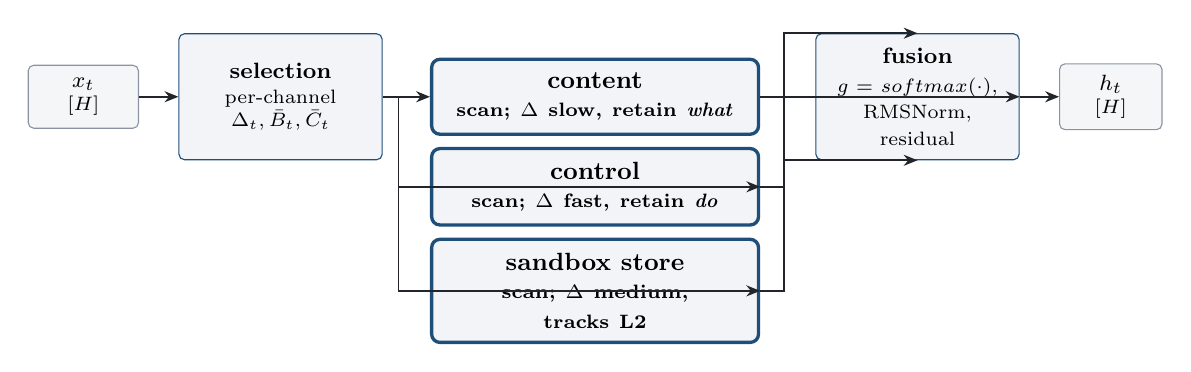
\begin{tikzpicture}
  \node[ekbox, minimum width=14mm, minimum height=8mm] (x) {$x_t$\\[-1pt]\scriptsize$[\Hdim]$};

  % selection network
  \node[ekbox, right=5mm of x, text width=23mm, minimum height=16mm,
        draw=ekLone, fill=ekLone!6] (sel)
    {\textbf{selection}\\[1pt]\scriptsize per-channel\\[-1pt]
     \scriptsize $\Delta_t,\Btr_t,\Cdim_t$};
  \draw[ekflow] (x) -- (sel);

  % three stores
  \node[ekstageL, right=6mm of sel, text width=38mm, minimum height=8.5mm] (sc)
    {\textbf{content}\\[-1pt]\scriptsize scan; $\Delta$ slow, retain \emph{what}};
  \node[ekstageL, below=1.4mm of sc, text width=38mm, minimum height=8.5mm] (sctl)
    {\textbf{control}\\[-1pt]\scriptsize scan; $\Delta$ fast, retain \emph{do}};
  \node[ekstageL, below=1.4mm of sctl, text width=38mm, minimum height=8.5mm] (ssb)
    {\textbf{sandbox store}\\[-1pt]\scriptsize scan; $\Delta$ medium, tracks L2};

  \draw[ekflow] (sel) -- (sc);
  \draw[ekflow] (sel.east) -- ++(2mm,0) |- (sctl.east);
  \draw[ekflow] (sel.east) -- ++(2mm,0) |- (ssb.east);

  % fusion
  \node[ekbox, right=7mm of sc, text width=23mm, minimum height=16mm,
        draw=ekLone, fill=ekLone!6] (fus)
    {\textbf{fusion}\\[1pt]\scriptsize $g=\sm(\cdot)$, $\Rt$, residual};
  \draw[ekflow] (sc.east) -- ++(3mm,0) |- (fus.north);
  \draw[ekflow] (sctl.east) -- ++(3mm,0) |- (fus.east);
  \draw[ekflow] (ssb.east) -- ++(3mm,0) |- (fus.south);
  \node[ekbox, right=5mm of fus, minimum width=13mm, minimum height=8mm] (ht) {$h_t$\\[-1pt]\scriptsize$[\Hdim]$};
  \draw[ekflow] (fus) -- (ht);
\end{tikzpicture}
\caption{One step of the L1 block. A single input $x_t$ feeds a selection
network that emits per-channel step sizes; the three stores then integrate the
same token at deliberately different rates, which is what makes the layer
\emph{selective} rather than a fixed-rate recurrence. Each store is advanced by
its own parallel scan, the three outputs are combined by a learned gate and a
residual connection (Eq.~\eqref{eq:l1-fusion}), and the result is a
fixed-size state plus a $h_t$ that continues to stage T.}
\label{fig:l1stores}
\end{figure}

\noindent
The outputs are fused with learned per-channel weights and
a residual connection:
\begin{equation}
  h_t = \Rt\Bigl( \sum_{c} g^c_t \odot y^c_t + h^{\mathrm{in}}_t \Bigr),
  \qquad g = \sm\bigl(\mathrm{Linear}_{\mathrm{fuse}}(h^{\mathrm{in}}_t)\bigr),
  \label{eq:l1-fusion}
\end{equation}
with an output gate $y' = y \odot \mathrm{SiLU}(\mathrm{Linear}_{\mathrm{gate}}(x))$
applied per channel before fusion. We additionally emit a pooled
\emph{compressed} triple $\texttt{compressed} = [c_1; c_2; c_3] \in \mathbb{R}^{B \times 3d}$
for logging and for the bounded-memory verification of
Section~\ref{sec:rq1}; this tensor is diagnostic only and never feeds
forward.

\subsubsection{Initialization}

\noindent
Following the S4D-Lin convention \cite{gu2022s4d} we set
$A_{\log,c} = \log(c)$ for channel $c = 1 \dots d$ and
$A_c = -\mathrm{softplus}(A_{\log,c})$, which spreads the time constants
geometrically so that different channels cover different memory horizons. The
step bias is set so that $\Delta \in [0.001, 0.1]$ at initialization (see the
error analysis above). Projections $B$ and $C$ use Xavier initialization, and
gates are zero-initialized so that every channel starts open---contribution
is added, not gated away, at step zero.

\subsubsection{Parallel scan versus recurrence, and the \texorpdfstring{$O(1)$}{O(1)} claim}

\noindent
Equations \eqref{eq:sel-a}--\eqref{eq:sel-rec} define a recurrence, but
training does not use it. Expanding the recurrence gives
\begin{equation}
  x^c_t = \sum_{s \le t} \Bigl(\prod_{s < r \le t} \Atr^c_r\Bigr) \Btr^c_s \odot u_s
  \; + \; \Bigl(\prod_{r \le t} \Atr^c_r\Bigr) \odot x^c_0 .
  \label{eq:scan-expansion}
\end{equation}
This is a first-order linear recurrence with input-dependent coefficients, so
it is computable by an associative scan in $O(T \log T)$ work (or $O(T)$ with a
sequential-but-batched formulation), fully parallel, with autograd flowing
through every term. At generation time the same equation is evaluated by
carrying the state: the model holds $x^c \in \mathbb{R}^{B \times d}$ per
channel, a \emph{fixed} tensor independent of how many tokens have been
produced.

\noindent
This yields the precise version of the ``$O(1)$ inference'' claim, which we
state carefully because the loose version is wrong. The inference
\emph{state} is $O(1)$ in $T$. Total work and total attention memory are not:
stage T still performs $O(TW)$ attention work and holds an $O(W)$ KV window per
layer. What is eliminated is the \emph{unbounded, per-token} cache and the
quadratic training cost. \emph{Remark:} the honest summary is ``bounded state,
linear training, windowed attention'', not ``constant cost''.

\subsection{Stage T: dense Transformer stack}

\noindent
$N_T$ identical blocks ($N_T = 3/5/6$ for the design sizes XS/S/M, $12$ as built), each pre-norm:
\begin{equation}
  \begin{aligned}
  u_1 &= \Rt(x) + \mathrm{PE}, &
  x &\leftarrow x + \mathrm{GQA}\bigl(u_1\bigr) \\
  u_2 &= \Rt(x), &
  x &\leftarrow x + \mathrm{SwiGLU}\bigl(u_2\bigr),
  \end{aligned}
  \label{eq:t-block}
\end{equation}
with $\mathrm{PE}$ the rotary injection and GQA restricted to the window
$W$. All blocks are identical: no dense/sparse split, no sparse indexer, no
experts. The rationale is that at this scale (12--50M parameters) those mechanisms add
machinery without the capacity to exploit it, and every ablation we can afford
is better spent on the L2 question.

\subsection{Layer 2: the sandbox}

\subsubsection{Diverse initialization}

\noindent
$K$ trajectories are produced by $K$ distinct projections,
\begin{equation}
  T^{(k)}_0 = W_k\, \texttt{hT} + b_k, \qquad k = 1,\dots,K,
  \label{eq:l2-init}
\end{equation}
with $W_k$ mutually orthogonal and spread gains. Identical copies of
$\texttt{hT}$ would satisfy any agreement objective trivially while destroying
the diversity that motivates multiple paths \cite{liang2023divergent}; diverse
initialization is therefore load-bearing, not cosmetic, and we ablate
diverse-versus-copy initialization explicitly.

\subsubsection{Debate rounds}

\noindent
For round $r = 1,\dots,R$ and trajectory $k$, the trajectory reads the
others---not itself:
\begin{align}
  Q_k &= T^{(k)} W_Q, \qquad K_j = T^{(j)} W_K, \quad V_j = T^{(j)} W_V \quad (j \neq k) \nonumber\\
  \mathrm{read}_k &= \sm\!\Bigl(Q_k K_{-k}^{\top} / \sqrt{\hd}\Bigr) V_{-k} \label{eq:debate-read}\\
  \gamma_k &= \sigma\bigl(W_\gamma [\mathrm{read}_k \,;\, T^{(k)}] + b_\gamma\bigr) \nonumber\\
  T^{(k)} &\leftarrow (1 - \gamma_k) \odot T^{(k)} + \gamma_k \odot \mathrm{MLP}(\mathrm{read}_k). \label{eq:debate-revise}
\end{align}
The repair gate $\gamma_k$ lets a trajectory decline the crowd, which is
necessary for the debate to be able to correct rather than merely average. The
cross-attention in \eqref{eq:debate-read} is over $K-1 \le 7$ keys, so it is
negligible cost and needs no specialized kernel.

\subsubsection{Anchored gated descent}

\noindent
This subsection is the core technical contribution, and it exists because the
obvious design is provably inert.

\paragraph{The step.}
Define a token-conditioned anchor \emph{outside} the trajectory set, an energy
per trajectory, and a learned per-trajectory per-channel gate:
\begin{align}
  a_t &= W_a\, \texttt{hT}_t, \label{eq:agd-anchor}\\
  E_k &= \tfrac{1}{2}\bigl\|T^{(k)} - a_t\bigr\|_2^2, \label{eq:agd-energy}\\
  g_k &= \sigma\bigl(W_g [\,T^{(k)}; a_t\,] + b_g\bigr) \in (0,1)^H, \label{eq:agd-gate}\\
  T^{(k)} &\leftarrow T^{(k)} - \etadim\, g_k \odot \bigl(T^{(k)} - a_t\bigr), \qquad \etadim \approx \tfrac{0.5}{S}. \label{eq:agd-step}
\end{align}

\paragraph{Why this step is well posed.}
\begin{proposition}[Monotonicity of the gated step]
\label{prop:agd-monotone}
Under \eqref{eq:agd-step} with $0 \le \etadim g_k \le 2$, the energy
\eqref{eq:agd-energy} is non-increasing: $E_k^{\text{new}} \le E_k$, with
strict decrease whenever $\etadim g_k \in (0,2)$ and $T^{(k)} \neq a_t$.
\end{proposition}
\begin{proof}
Write $c = \etadim g_k \odot$ (elementwise) and $\delta = T^{(k)} - a_t$. Then
$T^{(k)}_{\text{new}} - a_t = (1-c)\odot\delta$, so
\begin{equation}
  E_k^{\text{new}} - E_k = \tfrac{1}{2}\bigl(\lVert (1-c)\delta\rVert^2 - \lVert \delta \rVert^2\bigr)
  = \tfrac{1}{2}\sum_d \bigl[(1-c_d)^2 - 1\bigr]\delta_d^2
  = \sum_d \bigl(c_d^2 - 2c_d\bigr)\,\frac{\delta_d^2}{2}.
\end{equation}
Each summand is $\le 0$ when $0 \le c_d \le 2$, and $<0$ when
$c_d \in (0,2)$ and $\delta_d \neq 0$.
\end{proof}

\noindent
\begin{remark}[What kind of descent this is]
\eqref{eq:agd-step} is \emph{gate-scaled (preconditioned) descent} on
$E_k$, not literally $-\etadim \nabla E_k$, and the two coincide only when
$g_k \equiv 1$. We use the word ``preconditioned'' throughout and never claim
exact gradient descent.
\end{remark}

\paragraph{Why the readout moves.}
Two independent mechanisms guarantee the consensus changes. First, the target
$a_t$ is \emph{external} to the trajectory set, so the update is not a
redistribution among trajectories. Second, the gate $g_k$ differs across $k$,
so the update is not a uniform linear map applied identically to all
trajectories. Either alone would suffice; together they make the consensus
$\bar T^{(S)}$ a genuine function of the backbone state.

\paragraph{The same heterogeneity is also what preserves spread.}
This second role is easy to miss. Write $T^{(k)} = a_t + \lambda_k\bigl(T^{(k)}_0 - a_t\bigr)$,
where $\lambda_k$ is the product of $1-\etadim g_k$ over the descent steps.
Were every $\lambda_k$ equal, the deviations from the consensus would scale by
$\lambda_k$ alone and $\texttt{trajectory\_variance}$ would decay as
$(1-\etadim)^{2S}$---precisely the $0.356$ of
Section~\ref{sec:defect1}, since $\etadim = 0.5/S$. When the $\lambda_k$
differ, however, one term survives and never contracts. With
$d_k = T^{(k)}_0 - \bar T_0$ and $u = \bar T_0 - a_t$,
$T^{(k)} - \bar T = \lambda_k d_k - \bar\lambda d + (\lambda_k - \bar\lambda)\,u$,
and the last term is proportional to $\mathrm{Var}_k(\lambda_k)$ and does not
decay at all. Heterogeneous gates therefore convert descent pressure into
persistent spread instead of collapse. Measured, $V_{\mathrm{pre}}$ retains
$0.356$ under identical gates, $0.396$ under a common gate $g \equiv 0.9$, and
$0.60$--$0.75$ under heterogeneous gates---the regime containing the healthy
run, which falls $1.95 \to 1.22$, a factor of $0.626$. Gate heterogeneity is
thus load-bearing twice over: it is what makes the readout move, and it is what
holds $\rhodim$ clear of the floor.

\noindent
Measured on the toy model of \texttt{28\_Worked\_Examples.md}: the consensus
moved by $\|\Delta \bar T\|_2 = 0.2295$, closing $0.2199$ of its distance to
the anchor, with per-trajectory deviation retention
$[0.827,\; 0.822,\; 0.744,\; 0.787]$---i.e.\ refinement that did not force
collapse. The inert peer-mean variant moved the consensus by exactly $0$.

\subsubsection{Consensus and readout}

\noindent
The consensus is the mean of the $K$ trajectories after the $S$ descent
steps (the default), or alternatively, at each position separately, the
lowest-anchor-energy trajectory $\arg\min_k \lVert T^{(k)}_t - a_t \rVert$.
The choice is made per position so that position $t$ never depends on later
tokens or on other examples in the batch. A single dense projection then
produces logits:
\begin{equation}
  y = \bar T^{(S)} \in \mathbb{R}^{B \times T \times H},
  \qquad \mathrm{logits} = y\, W_{\mathrm{vocab}} \in \mathbb{R}^{B \times T \times V},
  \label{eq:l2-readout}
\end{equation}
with $W_{\mathrm{vocab}}$ tied to the input embedding. The head is evaluated
once per micro-batch.

Figure~\ref{fig:sandbox} shows the whole of stage L2. The two halves are
deliberately asymmetric: the debate phase is \emph{horizontal} (trajectories
interact with each other and the anchor is not yet defined), whereas the
descent phase is \emph{vertical} (every trajectory moves toward the same
external anchor $a_t$). The anchor is what makes the second half capable of
changing the readout at all, which is the subject of
Section~\ref{sec:defect1}.

\begin{figure}[htbp]
\centering
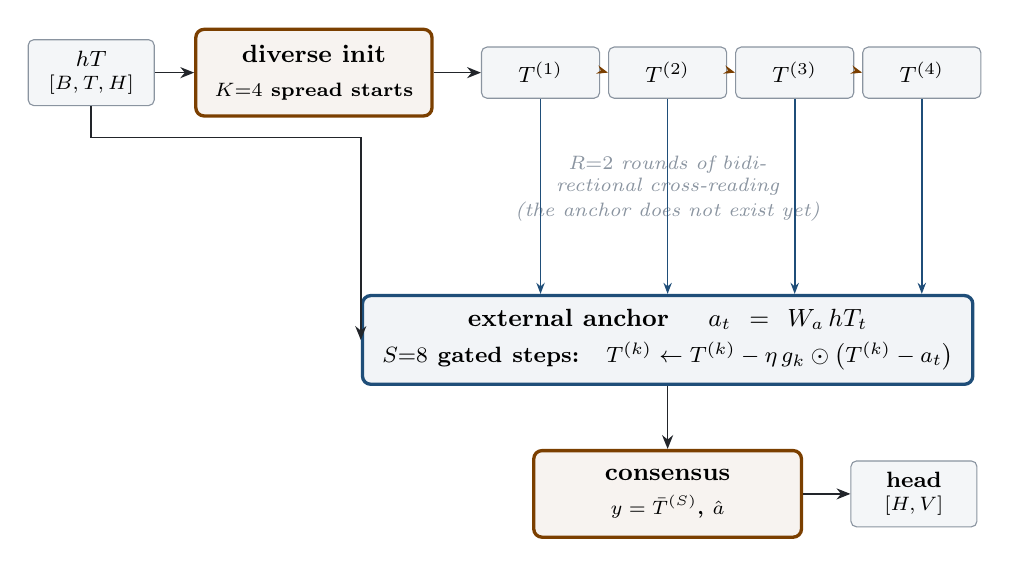
\begin{tikzpicture}
  % ---------- band 1: init and the K trajectories ----------
  \node[ekbox, minimum width=16mm, minimum height=8mm] (hT) {$hT$\\[-1pt]\scriptsize$[\Bdim,\Tdim,\Hdim]$};
  \node[ekstage2, right=5mm of hT, minimum width=30mm, minimum height=11mm] (init)
    {\textbf{diverse init}\\[1pt]\scriptsize $K{=}4$ spread starts};
  \node[ekbox, right=6mm of init, minimum width=15mm, minimum height=6.5mm] (t1) {$T^{(1)}$};
  \node[ekbox, right=1mm of t1, minimum width=15mm, minimum height=6.5mm] (t2) {$T^{(2)}$};
  \node[ekbox, right=1mm of t2, minimum width=15mm, minimum height=6.5mm] (t3) {$T^{(3)}$};
  \node[ekbox, right=1mm of t3, minimum width=15mm, minimum height=6.5mm] (t4) {$T^{(4)}$};
  \draw[ekflow] (hT) -- (init);
  \draw[ekflow] (init.east) -- (t1.west);

  % debate: bidirectional cross-reads along the row
  \draw[ekTwo, semithick, -{Stealth[length=4pt,width=3pt]}] (t1.east) to[bend left=16] (t2.west);
  \draw[ekTwo, semithick, -{Stealth[length=4pt,width=3pt]}] (t2.east) to[bend left=16] (t3.west);
  \draw[ekTwo, semithick, -{Stealth[length=4pt,width=3pt]}] (t3.east) to[bend left=16] (t4.west);

  % ---------- band 2: the debate annotation, centred and clear ----------
  \node[ektag, below=6mm of t2, text width=52mm, align=center] (deb)
    {$R{=}2$ rounds of bidirectional cross-reading\\[1pt]
     \scriptsize (the anchor does not exist yet)};

  % ---------- band 3: the anchor, carrying the update rule ----------
  \node[ekstageL, below=8mm of deb, text width=74mm, minimum height=11mm] (anc)
    {\textbf{external anchor} \quad $a_t = W_a\, hT_t$\\[2pt]
     \footnotesize $S{=}8$ gated steps:\quad
     $T^{(k)} \leftarrow T^{(k)} - \etadim\, g_k \odot \bigl(T^{(k)} - a_t\bigr)$};
  \draw[ekflow] (hT.south) -- ++(0,-4mm) -| (anc.west);

  % descent arrows: four distinct landing points on the anchor's top edge
  \foreach \k in {1,2,3,4}{
    \draw[ekLone, semithick, -{Stealth[length=4pt,width=3pt]}]
      (t\k.south) -- (anc.north -| t\k.center);
  }

  % ---------- band 4: consensus and head ----------
  \node[ekstage2, below=8mm of anc, minimum width=34mm, minimum height=11mm] (cons)
    {\textbf{consensus}\\[1pt]\scriptsize $y=\bar T^{(S)}$,\ $\hat a$};
  \node[ekbox, right=6mm of cons, minimum width=16mm, minimum height=8mm] (out)
    {\textbf{head}\\[-1pt]\scriptsize$[\Hdim,\Vdim]$};
  \draw[ekflow] (anc) -- (cons);
  \draw[ekflow] (cons) -- (out);
\end{tikzpicture}
\caption{Stage L2 in full. Diverse initialization separates $K$ trajectories;
the debate phase lets them read and revise each other ($R$ rounds, bidirectional
arrows) while the anchor does not yet exist. Only then is $a_t = W_a hT_t$
computed, and all $K$ trajectories descend toward that single external point for
$S$ steps under per-trajectory gates. The consensus and the agreement
diagnostic $\hat a$ leave as the M3 write-back.}
\label{fig:sandbox}
\end{figure}

\subsubsection{The three reported quantities}

\noindent
Three statistics ship with every forward pass. They are deliberately given
distinct names because conflating them is what made an earlier version of this
design undetectable.

\begin{description}
  \item[$\texttt{anchor\_energy}$, $E = \mathrm{mean}_{k,t} E_k$.] The
    quantity AGD descends. Reported as a monitor; \emph{never} used as a loss
    term, because minimizing it directly collapses every trajectory onto the
    anchor.
  \item[$\texttt{trajectory\_variance}$, $V_{\mathrm{pre}}$.] Mean squared
    distance of each trajectory to the consensus, measured \emph{after} the
    debate rounds and \emph{before} descent. This ordering matters: measuring
    after descent would report the effect of the descent rather than whether
    diversity survived cross-examination.
  \item[$\texttt{spread\_ratio}$, $\rhodim$.] Dimensionless: the
    ratio $\rhodim = V_{\mathrm{pre}} / \mathrm{mean}_{t,d}(\texttt{hT}_{t,d}^2)$,
    i.e.\ the fraction of backbone activation energy that the $K$ hypotheses
    still span. Because both numerator and denominator scale with activation magnitude,
    $\rhodim$ is comparable across width $H$, length $T$, and training scale.
    Collapse is $\rhodim \to 0$.
\end{description}

\subsection{The M3 write-back, and the causality rule (specified, not implemented)}
\label{sec:m3}

\noindent
Stage L2 is not a terminal head. After the consensus is formed, it emits a
feedback signal that is written into L1's third state store,
$S^{\mathrm{sandbox}}$:
\begin{equation}
  f_t = \mathrm{Linear}_{\mathrm{fb}}\bigl([\,y_t \,;\, V_t\,]\bigr),
  \qquad
  x^{3}_t = \Atr^{3}_t \odot x^{3}_{t-1} + \Btr^{3}_t \odot u_t + F \odot f_{t-1}.
  \label{eq:m3-writeback}
\end{equation}
This closes the loop between reasoning and memory: the sandbox can carry
tracking state and inject instructions into subsequent processing. Two
constraints are enforced and are not negotiable:

\begin{enumerate}
  \item \textbf{Causality.} Position $t$ reads only states at positions $<t$.
    The per-position state $m^3_t$ is the only thing stage L2 ever reads; the
    pooled $\texttt{compressed}$ triple is diagnostic and never feeds forward.
  \item \textbf{No cross-batch leakage.} During training, $f$ arrives
    \emph{detached} from the previous micro-batch. This is stated rather than
    hidden because the alternative silently conditions on future minibatch
    content.
\end{enumerate}

\subsection{Training objective}
\label{sec:loss}

\noindent
There are two training signals plus one supervision re-weighting term:
\begin{equation}
  \mathcal{L} \;=\; \lam_{\mathrm{lm}} \cdot \mathrm{CE}\bigl(\mathrm{shift}(\mathrm{logits}),\, \mathrm{shift}(\mathrm{labels})\bigr)
  \;+\; \lam_{\mathrm{ans}} \cdot \mathrm{CE}\bigl(\mathrm{logits}_{p-1},\, y\bigr)
  \;+\; \lam_{\mathrm{sbx}} \cdot \bigl[\max\bigl(0,\, \rhodim_{\min} - \rhodim\bigr)\bigr]^2,
  \label{eq:loss}
\end{equation}
with $\lam_{\mathrm{lm}} = 1.0$, $\lam_{\mathrm{sbx}} = 1.0$ (the shipped
configuration; the original design value was $0.1$), $\rhodim_{\min} = 0.05$.
The floor term exists only in the sandbox arm. Cross-entropy is causal and the
head runs once per micro-batch.

\noindent
The middle term re-weights the decision that is actually scored. In this task
the answer letter sits at position $p$ and is one token out of a median of
about 34 (MedMCQA) or 173 (MedQA), so plain language-model cross-entropy spends
roughly 97--99\% of its gradient on predicting question text. The extra term
applies the cross-entropy of the letter prediction at the same position and
metric as evaluation, with $\lam_{\mathrm{ans}} = 10$ in the campaign
recipe (and $0$ recovers the plain language-model loss). It is applied
identically to both arms.

\noindent
The second term is a \emph{floor}, not an agreement penalty. It is exactly
zero while the hypotheses retain at least $\rhodim_{\min}$ of the backbone's
spread, and grows only once they have collapsed. Verified numerically: a
healthy run ($\rhodim: 1.95 \to 1.22$) pays $0$; a collapsed run
($\rhodim = 10^{-6}$) pays $(0.05 - 10^{-6})^2 = 0.0025$.

Figure~\ref{fig:floor} plots the penalty. The shape is what justifies calling
it a floor rather than a regularizer: the function is identically zero across
four orders of magnitude of healthy spread, so it contributes no gradient at all
during normal training, and only the extreme right tail---where the hypotheses
have genuinely collapsed---is penalized. The penalty is also bounded, at
$(\rhodim_{\min})^2 = 0.0025$, so even total collapse cannot dominate the
cross-entropy term.

\begin{figure}[htbp]
\centering
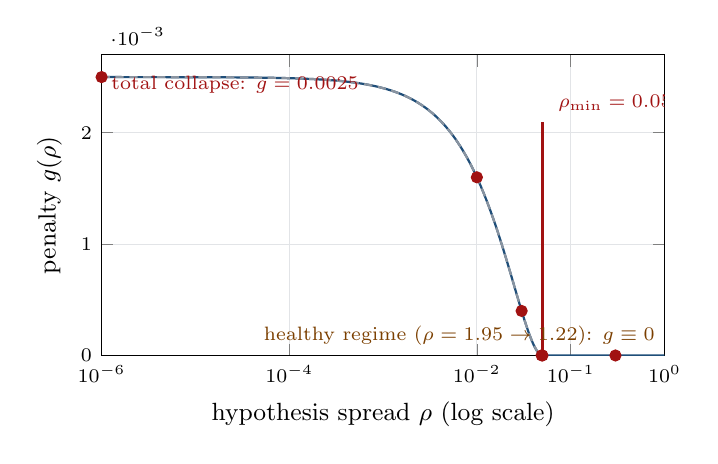
\begin{tikzpicture}
\begin{axis}[
  width=0.72\textwidth, height=5.4cm,
  xmode=log, xmin=1e-6, xmax=1, ymin=0, ymax=0.0027,
  xlabel={hypothesis spread $\rho$ (log scale)},
  ylabel={penalty $g(\rho)$},
  xtick={1e-6,1e-4,1e-2,1e-1,1}, grid=both, grid style={ekEdge!25},
  tick label style={font=\scriptsize}, label style={font=\small},
]
\addplot[ekLone, thick, domain=1e-6:1, samples=200]
  {max(0.0, 0.05 - x)^2};
\addplot[ekEdge, densely dashed, thick, domain=1e-6:0.05, samples=100]
  {max(0.0, 0.05 - x)^2};
\addplot[only marks, mark=*, mark size=2pt, ekWarn]
  coordinates {(1e-6,0.0025) (0.01,0.0016) (0.03,0.0004) (0.049,0.000001) (0.05,0) (0.3,0)};
\draw[ekWarn, thick] (axis cs:0.05,0) -- (axis cs:0.05,0.0021)
  node[above, font=\scriptsize, anchor=south west, xshift=2pt] {$\rhodim_{\min}=0.05$};
\node[font=\scriptsize, anchor=north west, text=ekWarn] at (axis cs:1e-6,0.0026)
  {total collapse: $g = 0.0025$};
\node[font=\scriptsize, anchor=north east, text=ekTwo] at (axis cs:1,0.00035)
  {healthy regime ($\rhodim = 1.95 \to 1.22$): $g \equiv 0$};
\end{axis}
\end{tikzpicture}
\caption{The spread floor $g(\rho) = [\max(0, \rhodim_{\min} - \rho)]^2$ on a
logarithmic spread axis. Solid blue is the penalty; the dashed segment marks the
region in which it is active. It is exactly zero for all
$\rho \ge \rhodim_{\min}$, so it injects no gradient while the hypotheses remain
distinct, and it saturates at $0.0025$ under complete collapse---two and a half
orders of magnitude below the $\lam_{\mathrm{lm}} = 1$ cross-entropy term, so it
can flag a collapse without being able to cause one.}
\label{fig:floor}
\end{figure}

\subsection{Complexity and parameter budget}

\paragraph{Cost.}
L1 training is $O(T)$ per channel with the associative scan
\eqref{eq:scan-expansion}; stage T is $O(TW)$ attention plus $O(T H I)$
feed-forward; L2 is
\begin{equation}
  O\bigl(R K T H^2 \;+\; R K^2 T H \;+\; S K T H\bigr),
  \label{eq:l2-cost}
\end{equation}
comprising the $K$ trajectory inits, the $3RK$ debate projections and the
single anchor projection (the $O(TH^2)$ terms), the $R$ rounds of $K$-way
cross-read at $O(K^2TH)$, and the gates of the $S$ descent steps at $O(SKTH)$.
The projection terms dominate whenever $H \gg K$: at configuration M
($H{=}512$, $K{=}4$, $S{=}8$, $R{=}2$) they are $128\times$ the cross-read
term, so counting only the $K^2$ attention work understates L2 by more than two
orders of magnitude. L2 is nonetheless linear in $T$ and quadratic only in the
tiny constant $K \le 8$.
Inference state is $3d$ per L1 channel plus an $O(W)$ KV window per T layer,
independent of tokens generated.

That constant-plus-window claim is easier to believe as a curve than as an
asymptotic, so Figure~\ref{fig:memory} plots the inference-side
state footprint against sequence length at configuration M. The windowed curve
is flat from $W = 512$ onward because $W$ is fixed; the full-attention curve is
the same curve with the window removed, and it is the only term that grows.

\begin{figure}[htbp]
\centering
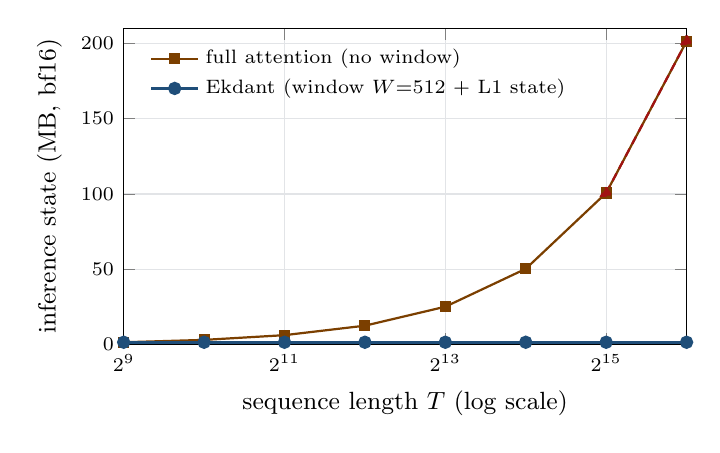
\begin{tikzpicture}
\begin{axis}[
  width=0.72\textwidth, height=5.6cm,
  xmode=log, xmin=512, xmax=65536, ymin=0, ymax=210,
  xlabel={sequence length $T$ (log scale)},
  ylabel={inference state (MB, bf16)},
  log basis x=2, xtick={512,2048,8192,32768},
  ytick={0,50,100,150,200}, grid=both, grid style={ekEdge!25},
  tick label style={font=\scriptsize}, label style={font=\small},
  legend style={font=\scriptsize, draw=none, fill=none, at={(0.03,0.97)}, anchor=north west},
  legend cell align=left,
]
\addplot[ekTwo, thick, mark=square*, mark size=1.6pt]
  coordinates {(512,1.57) (1024,3.15) (2048,6.29) (4096,12.58) (8192,25.17)
               (16384,50.33) (32768,100.66) (65536,201.33)};
\addlegendentry{full attention (no window)}
\addplot[ekLone, very thick, mark=*, mark size=1.8pt]
  coordinates {(512,1.58) (1024,1.58) (2048,1.58) (4096,1.58) (8192,1.58)
               (16384,1.58) (32768,1.58) (65536,1.58)};
\addlegendentry{Ekdant (window $W{=}512$ $+$ L1 state)}
\addplot[ekWarn, thick, densely dashed, mark=triangle*, mark size=2pt]
  coordinates {(32768,100.66) (65536,201.33)};
\node[font=\scriptsize, anchor=south west, text=ekWarn, xshift=3pt]
  at (axis cs:65536,201.33) {$127\times$};
\end{axis}
\end{tikzpicture}
\caption{Analytic projection of the inference-side state footprint at
configuration M of the \emph{full design with L1} ($H{=}512$, $N{=}4$ L1
layers, $N_{\mathrm{T}}{=}6$, $d_{\mathrm{state}}{=}256$, $2$ KV heads, bf16;
not the built model, whose cache is bounded by the window only). Ekdant holds flat at
$1.58$ MB: a $6$ KB L1 recurrent
state ($3 \cdot 256 \cdot 2$ bytes per L1 layer, over $N = 4$ layers) plus a
KV window that saturates at $W = 512$. Full attention over the same
tokens is $3$ KB per token, growing linearly without bound---$4.0$ times larger
at $T = 2048$ and $127$ times larger at $T = 65536$. Weights, activations and
the $K$-trajectory sandbox scratch space are excluded; the figure isolates the
one term the architecture is designed to make constant.}
\label{fig:memory}
\end{figure}

\paragraph{Parameters (as built).}
Embeddings are tied at $V \cdot H$. One T block costs approximately
$2.5H^2$ (grouped-query projections) $+\,3HI$ (SwiGLU with $I = 2H$), which
the code reproduces exactly (2{,}229{,}248 parameters per block at $H{=}512$).
The A/B pair differs only in L2:

\begin{center}
\small
\begin{tabular}{@{}lrr@{}}
\toprule
\rowcolor{ekHeadBG}\color{white}\textbf{Component} & \color{white}\textbf{Baseline (no L2)} & \color{white}\textbf{Sandbox} \\
\midrule
\rowcolor{ekEdge!12}Embeddings (tied) & 16.78M & 16.78M \\
\rowcolor{ekRowT}T ($N_T{=}12$) & 26.75M & 26.75M \\
\rowcolor{ekRow2}L2 & --- & 6.56M \\
\midrule
\rowcolor{ekEdge!25}\textbf{Total} & \textbf{43.53M} & \textbf{50.09M} \\
\bottomrule
\end{tabular}
\end{center}

\noindent
The comparison is therefore architecture-matched, not parameter-matched: the
sandbox arm has 15\% more parameters and runs $K{\times}R{\times}S$ extra
work per token. Counts are measured with \texttt{estimate\_model\_size}. L2 is
$2.3\times$ the closed-form estimate below ($6.56$M versus $2.8$M): the build
uses full $H{\times}H$ query/key/value cross-projections and an
$H\to2H\to H$ MLP, untied across rounds, which the estimate undercounted.
This is reported as a correction to the estimate, not as a change to the
architecture.

\paragraph{Parameters (design-time estimates for the full three-stage model).}

\begin{center}
\small
\begin{tabular}{@{}lrrr@{}}
\toprule
\rowcolor{ekHeadBG}\color{white}\textbf{Component} & \color{white}\textbf{XS ($H{=}256$)} & \color{white}\textbf{S ($H{=}320$)} & \color{white}\textbf{M ($H{=}512$)} \\
\midrule
\rowcolor{ekEdge!12}Embeddings (tied) & 8.4M & 10.5M & 16.8M \\
\rowcolor{ekRowL}L1 aSSM ($N{=}2/4/4$) & 1.5M & 4.8M & 13.0M \\
\rowcolor{ekRowT}T ($N_T{=}3/5/6$) & 1.7M & 4.4M & 13.4M \\
\rowcolor{ekRow2}L2 (init $+$ debate $+$ anchor $W_a$ $+$ gate $W_g$) & 0.8M & 1.3M & 2.8M \\
\rowcolor{ekEdge!12}Output head & tied & tied & tied \\
\midrule
\rowcolor{ekEdge!25}\textbf{Total} & \textbf{12.4M} & \textbf{21.0M} & \textbf{46.0M} \\
\bottomrule
\end{tabular}
\end{center}

\noindent
These design-time figures include L1 (not built) and a shallower T
($N_T{=}3/5/6$ versus $12$ as built); they are closed-form estimates and are
superseded by the measured table above for every result in this thesis.
The L2 figure rose from $0.6$/$1.0$/$2.2$M when the peer-mean step was
replaced by AGD, because the anchor $W_a \in \mathbb{R}^{H \times H}$ and gate
$W_g \in \mathbb{R}^{2H \times H}$ are new parameters; the budget increase is
the honest cost of the correction.

\subsection{Evaluated instantiation: pretrained backbone and gated add-on}
\label{sec:v2}

\noindent
The from-scratch pilot (Section~\ref{sec:results}) showed that a 50M model
trained only on MedMCQA learns the answer-letter prior and nothing a sandbox
could build on. The evaluated configuration therefore keeps stage L2 exactly as
specified above and changes what it sits on. The backbone is SmolLM2-135M
\cite{allal2025smollm2}: 30 layers, width $H=576$, 9 query and 3 key--value
heads, a 49{,}152-entry vocabulary and a tied output head. Let $h_t$ be its
final (normalised) hidden state. The sandbox arm applies L2 (consensus
$f$) through a per-channel gate $g\in\mathbb{R}^{H}$,
\begin{equation}
  h'_t = h_t + g \odot \bigl(\mathrm{RMSNorm}(f(h_t)) - h_t\bigr),\qquad g = 0 \text{ at initialisation},
  \label{eq:gated-addon}
\end{equation}
and the backbone's own head maps $h'_t$ to logits. With $g=0$ every arm
reproduces the pretrained model exactly, so any later difference is caused by
training the add-on; the mean $|g|$ shows how much the model chooses to use it.
The gated residual also removes the handicap of the pilot, where the consensus
replaced the backbone state. The consensus is normalised before the gate
because $h_t$ has already passed the backbone's final normalisation and goes
straight to the head: without it, the first sandbox run let the L2 output grow
the logits without bound and diverged (loss in the thousands, gradient norm
above $10^{11}$), a failure the pilot avoided by normalising after L2.

\begin{center}
\small
\begin{tabular}{@{}lll@{}}
\toprule
\rowcolor{ekHeadBG}\color{white}\textbf{Arm} & \color{white}\textbf{$f(h)$} & \color{white}\textbf{Parameters (measured)} \\
\midrule
Baseline & none ($h'=h$) & 134{,}515{,}008 \\
Sandbox & L2 consensus, $K{=}4$, $R{=}4$, MLP $4\times$, $S{=}8$ & 154{,}107{,}648 ($+19{,}592{,}640$) \\
\bottomrule
\end{tabular}
\end{center}

\noindent
L2 is scaled to the share of the model it had in the pilot (13.1\%): four
debate rounds with a debate MLP of width $4H$ give 12.7\%, whereas the pilot's
two rounds of width $2H$ would give 5.8\% at this width. Since
every L2 operation is per position, decoding reuses the backbone's key--value
cache and applies the add-on to each new token's state.

% =====================================================================
\section{Design audit: four defects found and fixed}
\label{sec:audit}

\noindent
This section reports defects found in our own design during review. Each is
given as a proposition with proof, a numerical demonstration, and a retained
ablation. None is described as a limitation of the approach in general; all
four are limitations of an earlier version of \emph{this} approach, found before
the main runs.

\subsection{Defect 1: the energy loop was readout-invariant}
\label{sec:defect1}

\noindent
The initial design descended each trajectory toward the running mean of the
trajectories:
\begin{equation}
  T^{(k)} \leftarrow (1-\etadim)\, T^{(k)} + \etadim\, \bar T,
  \qquad \bar T = \frac{1}{K}\sum_{j} T^{(j)}.
  \label{eq:peer-mean}
\end{equation}
This is a very natural thing to write, and it is useless.

\begin{proposition}[Peer-mean descent is mean-preserving]
\label{prop:peer-inert}
Under \eqref{eq:peer-mean} with common step $\etadim$ and \emph{any}
doubly stochastic mixing matrix $A$, that is
$y^{(k)} = \sum_j A_{kj}T^{(j)}$ with $\sum_j A_{kj} = 1$ and $\sum_k A_{kj} = 1$, the mean
$\bar T$ is invariant. In particular $\bar T_{\text{new}} = \bar T$, so any
readout that depends only on $\bar T$ is unchanged.
\end{proposition}
\begin{proof}
Average \eqref{eq:peer-mean} over $k$ with common $\etadim$:
\begin{equation}
  \bar T_{\text{new}} = (1-\etadim)\bar T + \etadim \bar T = \bar T .
  \label{eq:peer-inv}
\end{equation}
More generally, for $y^{(k)} = \sum_j A_{kj}T^{(j)}$ with row sums $1$, we get
$\bar T_{\text{new}} = (1-\etadim)\bar T + \etadim \bar T$ by
\emph{double stochasticity}: averaging the targets gives
$\frac{1}{K}\sum_k y^{(k)} = \sum_j \bigl(\frac{1}{K}\sum_k A_{kj}\bigr) T^{(j)} = \sum_j \frac{1}{K}T^{(j)} = \bar T$, using column sums $1$.
\end{proof}

\noindent
\begin{remark}[The precise form, because the loose form is false]
It is \emph{not} true that any uniform pull toward any linear function of the
trajectories is mean-preserving. For a general step
$T^{(k)} \leftarrow T^{(k)} + \etadim (y^{(k)} - T^{(k)})$ we get
\begin{equation}
  \bar T_{\text{new}} = \bar T + \etadim\bigl(\bar y - \bar T\bigr),
  \label{eq:general-step}
\end{equation}
so the consensus moves \emph{unless} $\bar y = \bar T$. Column sums equal to
$1$ is exactly the condition guaranteeing that, and leave-one-out mixing
$(J-I)/(K-1)$ satisfies it---which is why every peer-mean variant collapses
onto the same inert fixed point. A non-doubly-stochastic $A$ gives
$\bar y \neq \bar T$ and the readout \emph{does} move. Design rule: the descent
target must be external to the trajectory set, as $a_t$ is in
\eqref{eq:agd-anchor}, or a non-linear function of it, as the gate is.
\end{remark}

\paragraph{Consequences, measured.}
Because the head reads only the consensus \eqref{eq:l2-readout},
$\mathrm{logits}(S{=}0) = \mathrm{logits}(S{=}8)$ \emph{exactly}---gradient
descent that provably cannot change the output. Meanwhile the spread decays
like $(1-\etadim)^{2S} = 0.356$ at the configured
$\etadim = \tfrac{0.5}{S} = 0.0625$, $S = 8$: the model
became less diverse while producing bit-identical logits. A pure accuracy
comparison at $S = 0$ versus $S = 8$ would have shown ``no effect'' and been
interpreted as evidence that sandbox refinement does not help, when the truth
is that the mechanism was disconnected from the output.

Figure~\ref{fig:agd-vs-peer} makes the asymmetry visible. Both panels matter,
and the point is precisely that the obvious diagnostic fails. Energy---the
quantity the refinement optimizes---falls in \emph{both} variants, and the
inert peer-mean variant actually falls \emph{faster}. What distinguishes them is
the readout: AGD moves the consensus toward the anchor, while peer-mean leaves
it bit-identical forever, because averaging a fixed set of trajectories is a
fixed point of the step. So ``energy went down'' would have certified the broken
variant as the more successful one.

\begin{figure}[htbp]
\centering
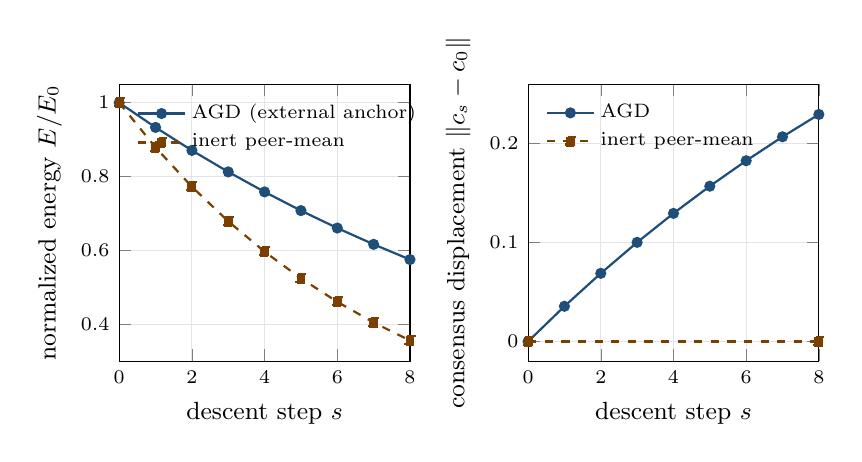
\begin{tikzpicture}
\begin{groupplot}[
  group style={group size=2 by 1, horizontal sep=1.5cm},
  width=0.435\textwidth, height=5.1cm,
  xlabel={descent step $s$},
  xmin=0, xmax=8, xtick={0,2,4,6,8},
  grid=both, grid style={ekEdge!25},
  tick label style={font=\scriptsize}, label style={font=\small},
  legend style={font=\scriptsize, draw=none, fill=none,
                at={(0.03,0.97)}, anchor=north west},
  legend cell align=left,
]
\nextgroupplot[
  ylabel={normalized energy $E/E_0$}, ymin=0.3, ymax=1.05,
]
\addplot[ekLone, thick, mark=*, mark size=1.6pt]
  coordinates {(0,1.0000) (1,0.9332) (2,0.8709) (3,0.8128) (4,0.7586)
               (5,0.7079) (6,0.6607) (7,0.6166) (8,0.5754)};
\addlegendentry{AGD (external anchor)}
\addplot[ekTwo, thick, dashed, mark=square*, mark size=1.6pt]
  coordinates {(0,1.0000) (1,0.8789) (2,0.7725) (3,0.6789) (4,0.5967)
               (5,0.5245) (6,0.4610) (7,0.4051) (8,0.3561)};
\addlegendentry{inert peer-mean}

\nextgroupplot[
  ylabel={consensus displacement $\lVert c_s-c_0\rVert$}, ymin=-0.02, ymax=0.26,
]
\addplot[ekLone, thick, mark=*, mark size=1.6pt]
  coordinates {(0,0.0000) (1,0.0356) (2,0.0689) (3,0.1002) (4,0.1295)
               (5,0.1570) (6,0.1827) (7,0.2069) (8,0.2295)};
\addlegendentry{AGD}
\addplot[ekTwo, thick, dashed, mark=square*, mark size=1.6pt]
  coordinates {(0,0.0000) (8,0.0000)};
\addlegendentry{inert peer-mean}
\end{groupplot}
\end{tikzpicture}
\caption{The central ablation, $S = 8$, $\etadim = 0.5/S$, gates
$g \in \{0.55, 0.60, 0.48\}$. \textbf{Left:} optimized energy decreases in
both variants, and faster for the broken one---energy alone cannot detect the
disconnection. \textbf{Right:} only the readout differs. AGD contracts the
consensus toward the fixed anchor, displacing it by $0.2295$; the inert
peer-mean preserves the mean exactly, so its curve is identically zero and its
logits are bit-identical to $S = 0$. This is why the ablation is reported as a
retained contrast rather than removed: it is the cheapest demonstration that a
refinement mechanism must be connected to the output to be measurable at all.}
\label{fig:agd-vs-peer}
\end{figure}

\paragraph{Fix and retained ablation.}
AGD \eqref{eq:agd-step} replaces \eqref{eq:peer-mean}; the anchors are external
and the gates differ across $k$, so by \eqref{eq:general-step} the consensus
moves. The inert variant is \emph{retained} as a reported contrast ablation
rather than deleted, because it is the cleanest available demonstration that
a refinement mechanism must be connected to the readout to be measurable.

\subsection{Defect 2: the agreement loss was minimized by collapse}
\label{sec:defect2}

\noindent
The initial second loss term was an agreement penalty $\lambda C$, where
$C$ was the mean squared deviation of trajectories from their consensus.

\begin{proposition}[The agreement penalty is minimized at zero spread]
\label{prop:agreement-degenerate}
Let $T^{(1)},\dots,T^{(K)} \in \mathbb{R}^H$ and
$C = \frac{1}{K}\sum_k \lVert T^{(k)} - \bar T\rVert^2$ with
$\bar T = K^{-1}\sum_k T^{(k)}$. Then $C = 0$ if and only if all trajectories
are identical. Consequently $\min C = 0$ is attained by collapse, and
$\partial C/\partial T^{(k)}$ points toward the consensus, so gradient
descent on $C$ has a zero-spread stationary point that is a global minimum.
\end{proposition}
\begin{proof}
$\lVert \cdot\rVert^2 \ge 0$ with equality iff the argument is $0$; hence $C$
is a sum of non-negative terms and vanishes exactly when every
$T^{(k)} = \bar T$, which forces all $T^{(k)}$ equal. For differentiability,
$\frac{\partial C}{\partial T^{(k)}} = \frac{2}{K}(T^{(k)} - \bar T) - \frac{2}{K^2}\sum_j (T^{(j)} - \bar T) = \frac{2}{K}(T^{(k)} - \bar T)$, which is $0$ precisely at
$T^{(k)} = \bar T$ and points inward toward it otherwise.
\end{proof}

\noindent
This is the transfer of the RL collapse mechanism
(Section~\ref{sec:rl-collapse}) into our loss: the penalty is a collapse
detector that the optimizer is rewarded for defeating. The fix
\eqref{eq:loss} inverts the direction of the constraint, from ``penalize
disagreement'' to ``penalize the \emph{absence} of disagreement'', which has
its minimum at a healthy spread.

\begin{proposition}[The floor is non-degenerate]
\label{prop:floor-nondegenerate}
For $\rhodim > 0$ the term $g(\rhodim) = [\max(0, \rhodim_{\min} - \rhodim)]^2$
satisfies $g(\rhodim) = 0$ for all $\rhodim \ge \rhodim_{\min}$, is strictly
decreasing on $(0, \rhodim_{\min}]$, and $g(\rhodim) \to \rhodim_{\min}^2 > 0$
as $\rhodim \to 0$. Hence its global minimum is attained on the
\emph{non-collapsed} set $\{\rhodim \ge \rhodim_{\min}\}$, not at collapse.
\end{proposition}
\begin{proof}
Immediate: for $\rhodim \ge \rhodim_{\min}$ the inner maximum is $0$, so
$g \equiv 0$; on $(0,\rhodim_{\min}]$ the inner term is
$\rhodim_{\min} - \rhodim \ge 0$, strictly decreasing in $\rhodim$, so $g$ is
strictly decreasing there with supremum $\rhodim_{\min}^2$ at $\rhodim = 0^+$.
\end{proof}

\noindent
One honest caveat: the floor constrains only the \emph{lower} bound on spread.
It does not push trajectories apart when $\rhodim \ge \rhodim_{\min}$, so it
is a collapse guard rather than a diversity objective. This is intentional,
since an active diversity term is exactly the term that risks trading
correctness for disagreement. It is also why $\rhodim_{\min}$ appears in the
ablation grid.

\subsection{Defect 3: the evaluation plan was not measurable at this scale}
\label{sec:defect3}

\noindent
RQ2 and RQ3 were originally specified on GSM8K and HumanEval. At 12--46M
parameters these tasks sit at chance: the smallest model reported to exceed
$80\%$ on GSM8K is 34B, and 1.3B plus a trained verifier was needed to reach
$81.5\%$ \cite{li2023tinygsm}. A pre-registered comparison on a
floor-performing benchmark cannot decide anything; it can only return noise
that will be over-interpreted. The fix is a strict separation between a
\emph{runnable} decision set (perplexity, ARC-easy, HellaSwag, LAMBADA, and
synthetic known-answer multi-step items) and a \emph{scaling-held-out} set
(GSM8K, HumanEval, MMLU) that is reported but never used as a gate
(Section~\ref{sec:eval}). The built evaluation narrows the runnable set
further to letter-accuracy on medical multiple-choice questions (MedMCQA and
MedQA), where a 50M model can at least reach above-chance accuracy.

\subsection{Defect 4: an ambiguous discretization convention}

\noindent
Our own worked example cited the specification as using exact ZOH while in
fact computing the first-order form, an inconsistency worth $43\%$ on that
example. The resolution and the error analysis are in
Section~\ref{sec:discretization}. The general lesson, applied to the rest of
this document, is that a specification and an implementation must agree on
which convention is in force before any number derived from either is quoted.

% =====================================================================
\section{Data}
% =====================================================================

\noindent
The evaluated configuration (Section~\ref{sec:v2}) uses two public generative
medical datasets, in sequence and never jointly.

\paragraph{PubMedQA.}
\texttt{qiaojin/PubMedQA}, configuration \texttt{pqa\_artificial}
\cite{jin2019pubmedqa}: 211{,}269 research questions, each with the abstract
of a PubMed article and the article's conclusion. A seeded draw holds out
2{,}000 rows; the other 209{,}269 train phase~1 (question and abstract
$\to$ conclusion). Measured with the SmolLM2 tokenizer, an abstract has median
324 and 99th-percentile 627 tokens and a conclusion median 47 and
99th-percentile 130, about 85M tokens per epoch.

\paragraph{MedQuAD.}
\texttt{keivalya/MedQuad-MedicalQnADataset} \cite{benabacha2019medquad}:
16{,}407 consumer-health question--answer pairs from NIH websites, with
14{,}345 unique questions (3{,}474 rows share a question). The split is by
unique question, so rows sharing a question always land together: a seeded
permutation of the questions assigns half to the benchmark, scored once and
never trained on or used for selection, and half to fine-tuning, of which
10\% of the questions are held back to choose the checkpoint. Answers have
median 182 and maximum 5{,}646 tokens; they are cut at 512 tokens, which keeps
89\% of them whole.

\paragraph{Prompts and loss.}
Prompts are \texttt{Question: \{q\}} followed by \texttt{Context: \{abstract\}}
for PubMedQA, then \texttt{Answer:}; the target is the answer followed by the
end-of-sequence token. The loss and every perplexity cover the answer tokens
only. Sequences are capped at 1{,}024 tokens by trimming the abstract, never
the answer.

\paragraph{Pilot data (from-scratch build).}
The pilot (Section~\ref{sec:results}) used two medical multiple-choice
datasets, in sequence and never jointly, described in the rest of this
section.

\paragraph{MedMCQA.}
\texttt{openlifescienceai/medmcqa}: 182{,}822 training rows, of which 326 carry
no label, leaving \textbf{182{,}496 labelled rows} used for phase~1, and a
labelled validation split of 4{,}183 rows, of which 4{,}170 remain after dropping 13 rows whose
question is shorter than 12 characters. The public test split ships
\texttt{cop}$=-1$ for every row (no released labels) and is therefore
\emph{never scored}; an earlier version of the evaluator did score it and
reported nothing more than each model's rate of predicting ``A''
(Known Issues T18). The validation split is never trained on and doubles as
the checkpoint-selection set.

\paragraph{MedQA.}
\texttt{GBaker/MedQA-USMLE-4-options}: 10{,}178 training rows and 1{,}273
official test rows. A seed-locked permutation of the training rows gives a
\textbf{60\% fine-tuning partition (6{,}106 rows)} and a complementary
\textbf{40\% benchmark partition (4{,}072 rows)} that is never trained on and
scored once. The official test split is also untouched. The same seed yields
the identical partition for both arms.

\paragraph{Prompt and target.}
Every example is rendered as the question, four lettered options, and the
string \texttt{Answer:}; the training target is the letter token that follows.
Evaluation reads the logits at the single position that predicts that token
and takes the argmax over the four letter tokens, so no free-form generation or
option re-scoring is involved.

\paragraph{Lengths.}
Measured with the trained tokenizer, MedMCQA examples have median 34 and
99th-percentile 118 tokens; MedQA examples have median 173, 99th-percentile 364
and maximum 857 tokens. None of the 198{,}000 rows exceeds the 2048-token
limit, so nothing is truncated or dropped. Batches are padded to the batch
maximum.

\paragraph{Tokenizer.}
A byte-pair-encoding vocabulary \cite{sennrich2015bpe} with a $32{,}768$-entry
budget is
trained once on 20{,}000 MedMCQA training prompts (NFD-normalised, lower-cased,
whitespace pre-tokenised) and then reused for the second phase and for both
arms, so the comparison is not confounded by tokenization. On this sample the
trainer learns $26{,}766$ entries; the embedding table keeps the full budget, so
$6{,}002$ rows ($3.07$M parameters, identical in both arms) are never used and
are included in the parameter counts.

% =====================================================================
\section{Training}
\label{sec:training}
% =====================================================================

\noindent
\textbf{Evaluated configuration.} Both arms share one recipe and one
data order, so L2 is the only variable: AdamW with two learning-rate
groups (backbone $5\times10^{-5}$; add-on and gate $10^{-3}$, without weight
decay on the gate), a cosine schedule per phase with 200 warm-up steps,
gradient clipping at $1.0$, bf16 autocast on A100 GPUs, and an effective batch
of 32 sequences. Phase~1 is one epoch of PubMedQA, validated on the 2{,}000
held-out rows every quarter of the epoch; phase~2 is three epochs of the
MedQuAD fine-tuning half, validated each epoch. The final checkpoint is the
better of the best and the last phase-2 checkpoint on the validation
questions. Each arm runs on its own GPU; the seed is 17.

\noindent
\textbf{Pilot recipe.} Both pilot arms shared one recipe, so the presence of
L2 was the only variable. The campaign recipe (see the runbook
\texttt{run.md}, Part~B) is:

\begin{center}
\small
\begin{tabular}{@{}>{\raggedright\arraybackslash}p{0.34\linewidth}>{\raggedright\arraybackslash}p{0.56\linewidth}@{}}
\toprule
Setting & Value \\
\midrule
Phase 1 & all of MedMCQA, 100 epochs, learning rate $3\times10^{-4}$, cosine
  decay \cite{loshchilov2016sgdr}, 200 warmup steps \\
Phase 2 & 60\% of MedQA, 10 epochs, learning rate $5\times10^{-5}$ with its own
  cosine schedule and warmup \\
Optimizer steps & $381{,}480$ in total ($3{,}802$ per phase-1 epoch $\times 100$
  plus $128$ per phase-2 epoch $\times 10$) \\
Effective batch & $48$ sequences (batch $6$ $\times$ accumulation $8$ on one
  16\,GB T4) \\
Optimizer & AdamW, decoupled weight decay $0.1$, $\beta=(0.9,0.95)$
  \cite{loshchilov2017adamw} \\
Gradient clipping & $1.0$ \\
Dropout & $0.1$ (embedding) \\
Precision & bf16 autocast where supported, fp16 with loss scaling otherwise
  (the T4 has no bf16) \\
Answer-letter weight & $\lam_{\mathrm{ans}}=10$ (Equation~\ref{eq:loss}) \\
Sequence length & at most $2048$, padded to the batch maximum \\
Seed & $17$ (also fixes the 60/40 MedQA partition) \\
Hardware & $1\times$ T4, no distributed strategy \\
\bottomrule
\end{tabular}
\end{center}

\noindent
Two knobs exist purely to prevent memorisation of the small MedQA fine-tune
set: the phase-2 learning rate and the phase-2 epoch cap. A pre-protocol
40-epoch pilot that replayed the phase-1 epoch count over the MedQA training
set (all 10{,}178 rows) at the full learning rate drove training
cross-entropy to about $0.05$ while held-out accuracy stopped improving, and
the legacy 100-epoch run did the same on the 6{,}106-row partition (Known
Issues T21); the answer-letter weight
addresses the separate dilution of the decision signal (T22). Both are applied
to both arms. The phase-1 schedule restarts for phase~2, and a trailing
partial gradient-accumulation group is flushed at the end of every epoch
(T23).

\noindent
Phases run strictly in order: train on MedMCQA, record the MedMCQA validation
score, fine-tune on the 60\% MedQA partition, then benchmark. The checkpoint
that runs the final benchmark is the better of the best phase-2 checkpoint and
the last checkpoint, judged on the untouched MedMCQA validation split, so the
benchmark rows are never used for selection. A smoke test (a few hundred rows,
one epoch, with save, resume and evaluation) and the 141-test unit suite must
pass before any full run.

% =====================================================================
\section{Evaluation protocol}
\label{sec:eval}

\subsection{Principle: cost-matched, and pre-registered}

\noindent
Every comparison in this thesis is fixed before the run. Three comparisons are
mandatory for any sandbox claim, and reporting only the first is considered a
failed evaluation:
\begin{enumerate}
  \item sandbox versus greedy decoding;
  \item sandbox versus self-consistency majority vote \cite{wang2022sc} at
    equal FLOPs and equal token budget;
  \item \textbf{sandbox versus a depth-matched model with no sandbox}, at the
    same parameter count and the same block-pass budget.
\end{enumerate}
The third control exists because of Section~\ref{sec:counter-evidence}: when
compute is moved into extra layers rather than into a refinement mechanism,
depth often wins, and without this control the two are indistinguishable.
The A/B actually run in this thesis is the weaker no-sandbox comparison at
equal architecture; the first two comparisons concern generative decoding,
which the letter-logit protocol does not use, and the depth- or
parameter-matched control is open work.

\subsection{Validation and test harness}

\noindent
Correctness is gated by a $141$-test CPU unit suite
(\texttt{09-Code/tests}) covering the model, the sandbox, the Transformer
stack, the data pipeline, the learning-rate schedule and the seed-locked
evaluation split, and by a one-epoch smoke run of each arm that exercises
training, resume and evaluation end to end. Held-out evaluation can be re-run
on a saved checkpoint without training (\texttt{--eval-only}).

\subsection{RQ1: memory (protocol for future work)}
\label{sec:rq1}

\noindent
\emph{These checks require L1 and are not run in this thesis.}

\begin{enumerate}
  \item \textbf{Bounded-state proof.} Forward passes at
    $T = 512 / 2048 / 4096$ must produce identical \texttt{compressed} shapes
    $[B, 3d]$ and flat peak memory ($\pm5\%$), with tokens per second reported
    against the exact-attention baseline at each length \cite{dao2022flashattn}.
  \item \textbf{Mechanism checks.} Selective-copying accuracy and
    induction-style extrapolation, where selective dynamics must clearly beat
    static gating---if they do not, L1's core premise fails.
  \item \textbf{Backbone ablation.} L1 versus a small Transformer at equal
    parameters and equal tokens: perplexity, throughput, memory versus length.
  \item \textbf{Recall probe.} One exact-recall task where attention is
    expected to win, reported as the bounded limitation.
\end{enumerate}

\subsection{RQ2: reasoning}

\noindent
\textbf{Evaluated configuration.} The primary measure is the perplexity of
the reference answer on the MedQuAD benchmark half (mean negative
log-likelihood over answer tokens), measured before training, after phase~1
and at the end, and broken down by question type because many MedQuAD answers
follow fixed templates. Arms are compared by a paired bootstrap
\cite{koehn2004bootstrap} over questions (1{,}000 resamples): a difference
counts only if its 95\% interval excludes zero. ROUGE-L \cite{lin2004rouge}
and token F1 on 1{,}000 greedily generated answers report whether the content
of written answers changes, and perplexity on the PubMedQA held-out rows after
the fine-tune measures forgetting.

\noindent
\textbf{Pilot.} All scoring is letter-accuracy on held-out multiple-choice rows.
The reference floor is not $25\%$: the gold letters are unbalanced, so a
model that always outputs the most common letter scores $32.11\%$ on MedMCQA
validation (always A), $25.69\%$ on the MedQA benchmark partition (always B)
and $27.73\%$ on the MedQA test split (always A). Every evaluation records
the predicted-letter counts and this majority rate, and results are read
against it. The decision gate is the MedQA 40\% benchmark partition
(\texttt{medqa\_bench}, 4{,}072 rows, scored once), with the official MedQA
test split (1{,}273 rows) as a second untouched number. The MedMCQA validation
split (4{,}170 usable rows) is the selection set, and its phase-1 versus final values
measure how much the MedQA fine-tune erodes MedMCQA. Open-ended benchmarks
(GSM8K, HumanEval, MMLU) are out of scope at this scale
(Section~\ref{sec:defect3}).

\noindent
Ablations, each mapped to a knob: $K \in \{1,4,8\}$ (with $K{=}1$ the
chain-of-thought control); $R \in \{0,2,3\}$; $S \in \{0,4,8\}$ (with
$S{=}0$ the inert-mechanism control of Section~\ref{sec:defect1}); diverse
versus copy initialization; mean versus lowest-anchor-energy consensus;
$\rhodim_{\min} \in \{0.01, 0.05, 0.2\}$; and \textbf{anchor versus peer-mean}
target, which isolates the correction of Defect~1.

\subsection{RQ3: honesty}

\begin{enumerate}
  \item \textbf{Calibration.} Agreement $\hat a = 1/(1+V)$ plotted against
    per-example accuracy, with expected calibration error reported. This is the
    measurement that decides whether consensus is a usable confidence signal.
    The sandbox's three diagnostics (\texttt{anchor\_energy},
    \texttt{trajectory\_variance}, \texttt{spread\_ratio}) are computed over
    real tokens only and persisted per epoch and per evaluation; the
    per-example agreement needed for the calibration plot is not yet
    exported, so RQ3 remains untested.
  \item \textbf{Collapse monitoring.} $\rhodim$ reported as a learning curve.
    A falling $\rhodim$ is the failure signal and must be visible in the
    training logs, not reconstructed afterwards.
  \item \textbf{Overturn accounting.} Per debate round, counts of
    wrong$\rightarrow$right versus right$\rightarrow$wrong transitions. Majority
    pressure suppressing corrections appears here first
    \cite{wu2025debate}.
  \item \textbf{Reranking.} Step-energy rerank versus final-vote, plus
    rationale-aware early stopping \cite{wan2025rasc} for the efficiency table.
\end{enumerate}

\subsection{Results}
\label{sec:results}

\noindent
\paragraph{Evaluated configuration (baseline complete, sandbox pending).}
The first baseline run (one seed, one A100, about 1\,h\,15\,min) is complete;
both arms are being re-run as a pair, and the table is updated from those
runs. Its reference-answer perplexity on the MedQuAD benchmark half fell from
$7.578$ before training to $3.782$ (8{,}258 answers), against $3.958$ on the
validation questions, so selection did not flatter the benchmark. On the
PubMedQA held-out rows, perplexity fell from $9.703$ to $7.534$ during
phase~1 and rose to $8.192$ after the MedQuAD fine-tune: some forgetting,
still well below the untrained model. The first sandbox run diverged
(Section~\ref{sec:v2}) and is being repeated with the normalised add-on.

\begin{center}
\small
\begin{tabular}{@{}lccccc@{}}
\toprule
\rowcolor{ekHeadBG}\color{white}\textbf{Arm} & \color{white}\textbf{Zero-shot ppl} & \color{white}\textbf{Benchmark ppl} & \color{white}\textbf{$\Delta$ vs.\ baseline (95\% CI)} & \color{white}\textbf{ROUGE-L / F1} & \color{white}\textbf{$|g|$} \\
\midrule
Baseline & 7.578 & 3.782 & --- & 0.316 / 0.380 & --- \\
Sandbox & \textit{[PENDING]} & \textit{[PENDING]} & \textit{[PENDING]} & \textit{[PENDING]} & \textit{[PENDING]} \\
\bottomrule
\end{tabular}
\end{center}

\noindent
The from-scratch pilot below is the reason for this configuration.

\paragraph{Pipeline-scale pilot (completed).}
A full 3-epoch A/B on a single T4 (full data, one seed, per-stage learning
rate) is the only completed head-to-head run. It predates the sequential
60/40 protocol, trained MedMCQA then MedQA jointly, and the MedQA stage was
only about 638 optimizer steps, so the MedQA column sits at chance. It is
reported as a pipeline check, not as a thesis result:

\begin{center}
\small
\begin{tabular}{@{}lrrr@{}}
\toprule
\rowcolor{ekHeadBG}\color{white}\textbf{Arm} & \color{white}\textbf{Params} & \color{white}\textbf{MedMCQA val (4{,}170)} & \color{white}\textbf{MedQA test (1{,}273)} \\
\midrule
Baseline (no L2) & 43.53M & 33.31\% & 25.69\% \\
Sandbox (L2) & 50.09M & 32.01\% & 26.08\% \\
\bottomrule
\end{tabular}
\end{center}

\noindent
The MedMCQA gap of 1.3 points is within about two noise standard deviations
($\sigma\approx0.7$ points), so the two arms are statistically
indistinguishable at this scale: a tie. Section~\ref{sec:counter-evidence}
pre-committed to reporting a tie if that is what the data show.

\paragraph{Legacy 100-epoch baseline (completed, one arm).}
A 100-epoch run of the baseline arm on the sequential protocol, but before the
phase-2 learning-rate and epoch caps existed (phase~2 also ran 100 epochs at
$3\times10^{-4}$), reached 33.33\% MedMCQA validation accuracy after
phase~1---no better than the 3-epoch run---with training cross-entropy at
$0.58$ against validation cross-entropy at $4.61$. Its selected checkpoint
scored 26.89\% on the MedQA benchmark partition and 27.02\% on the official
MedQA test set, close to chance. The model memorised MedMCQA rather than
generalising from it. This is the evidence behind the phase-2 caps and the
answer-letter weight (Section~\ref{sec:training}), and the reason the phase-1
validation curve is now recorded every epoch: the number of phase-1 epochs
should be chosen from that curve before the sandbox arm is run.

\paragraph{Current recipe, 2 phase-1 epochs (baseline complete).}
With the capped fine-tune and the answer-letter weight, the phase-1
validation curve of a 20-epoch baseline peaked after the second epoch
($33.33\%$) and then fell while training loss kept dropping, so phase~1 was
cut to two epochs. The 2-epoch baseline reached $33.91\%$ on MedMCQA
validation after phase~1 (majority rate $32.11\%$), $25.44\%$ on the MedQA
benchmark partition (majority $25.69\%$) and $29.62\%$ on the MedQA test
split (majority $27.73\%$). Only the last clears its majority rate, by
$1.9$ points against a noise standard deviation of about $1.3$. At this
scale the backbone has learned little beyond the answer-letter prior. The
pilot's sandbox arm reached $32.23\%$ after phase~1 and then stopped on an
out-of-memory error caused by other jobs on a shared GPU; it was not re-run,
because the pilot was superseded by the evaluated configuration
(Section~\ref{sec:v2}).

\paragraph{Pending tables.}
The tables below are placeholders. They fix the required content and its
provenance in advance; no number is reported until the run produces it.

\begin{center}
\small
\begin{tabular}{@{}>{\raggedright\arraybackslash}p{0.34\linewidth}>{\raggedright\arraybackslash}p{0.56\linewidth}@{}}
\toprule
\rowcolor{ekHeadBG}\color{white}\textbf{Table} & \color{white}\textbf{Status} \\
\midrule
\rowcolor{ekRowW}
Campaign recipe (capped fine-tune, answer weight): \texttt{medqa\_bench}, \texttt{medqa\_test}, MedMCQA phase-1 $\to$ final & superseded by the evaluated configuration (Section~\ref{sec:v2}) \\
Cost report: parameters, tokens$\times K$, FLOPs, wall-clock & \textit{[PENDING]} \\
Depth- or parameter-matched control (no L2) & \textit{[PENDING]} \\
$K, R, S$ ablations & \textit{[PENDING]} \\
$\rhodim_{\min}$ sweep and anchor versus peer-mean & \textit{[PENDING]} \\
Agreement--accuracy calibration (RQ3) & \textit{[PENDING]} --- needs per-example agreement export \\
Multi-seed variance & \textit{[PENDING]} \\
Layer ladder: backbone-only $\to$ $+$L2 $\to$ $+$L1$+$L2 & \textit{[PENDING]} --- last step needs L1 \\
\bottomrule
\end{tabular}
\end{center}

% =====================================================================
\section{Prior art, and the strongest evidence against us}
\label{sec:counter-evidence}

\noindent
The novelty audit's most important finding is not a supporting citation. Rauba,
Fanconi and van der Schaar \cite{rauba2026trm} run a compute-matched ladder
from a plain Transformer to an autoregressive recursive model, holding block
design, token stream, objective, and total block-pass budget fixed, and report
that the full recursive variant shows \emph{no consistent benefit}. What
generalizes best is untied depth and a \emph{flat two-stream recurrent
baseline}.

\noindent
Three consequences, stated plainly:

\begin{enumerate}
  \item \textbf{Stage L2 cannot be justified by appeal to that line of work.}
    Its own conclusion cautions against investing in the mechanism. Any
    argument that leans on it as evidence that latent refinement helps would
    be using the paper against its finding.
  \item \textbf{The encouraging signal is structural, not mechanistic.} What
    worked there was separating streams and reading out with a weighted
    combination, which is closer to L2's shape than to nested halting---and is
    independently corroborated at comparable scale by the dual-stream result of
    Kerce et al.~\cite{kerce2026dualstream}. Two independent sources therefore support
    \emph{stream separation}, which is the part of stage L2 we defend. The
    \emph{recursive refinement} part is the hypothesis under test.
  \item \textbf{The bar for our ablation is higher than we originally set.} The
    informative control is depth-matched-no-sandbox, not sandbox-versus-greedy
    (Section~\ref{sec:eval}).
\end{enumerate}

\noindent
The expected result is correspondingly weaker than it was before this audit:
the honest prior from the best-matched study in our own library is \emph{no
reliable gain}. RQ2 is therefore written as a falsifiable question with a
genuine chance of a negative answer, and the thesis pre-commits to reporting a
tie.

% =====================================================================
\section{Limitations and threats to validity}
\label{sec:limitations}

\begin{description}
  \item[Scale.] At the 135M-parameter scale (and 50M in the pilot), absolute
    numbers will be far below published frontier results. The claims are about
    \emph{mechanisms} moving a metric, never about state-of-the-art quality.
  \item[Not parameter-matched.] The sandbox arm has $19.59$M more
    parameters than the baseline and does more work per token, so a gain could
    come from added capacity rather than from the debate mechanism. A
    same-size non-sandbox block would separate the two; it is not part of this
    evaluation and remains future work.
  \item[Pretrained backbone.] The evaluated L2 is an add-on to a model trained
    elsewhere on about two trillion tokens; a result says whether L2 helps
    such a model, not whether it helps a model trained from scratch, and the
    backbone's pretraining data cannot be audited for overlap with the medical
    test questions.
  \item[Generative metrics.] Perplexity rewards predicting the reference
    wording, and MedQuAD answers are partly templated; ROUGE-L and token F1
    reward surface overlap, not correctness. Per-type perplexity and the
    paired bootstrap limit, but do not remove, these weaknesses.
  \item[No L1.] The selective-SSM storage layer is specified but not
    built, so the memory claim (P1) and RQ1 are untested here. A fixed-size
    recurrent state is a lossy summary, and exact associative recall is
    expected to lose to attention \cite{lieber2024jamba}; the recall probe
    stays in the protocol for that follow-up.
  \item[Collapse and false consensus.] K trajectories agreeing can be jointly
    wrong. $\rhodim$ detects \emph{collapse}, not \emph{error}; a diverse but
    uniformly wrong set will not trip the floor. This is why RQ3 measures
    calibration rather than assuming agreement implies correctness.
  \item[Compute cost.] Stage L2 adds $K{=}4$ trajectories, $R$ debate
    rounds ($2$ in the pilot, $4$ in the evaluated configuration) and $S{=}8$
    descent steps per token \eqref{eq:l2-cost}; the
    sandbox arm is estimated at roughly $1.5\times$ the baseline's wall-clock
    on a T4 (not yet timed on a full run). Gains must be reported alongside parameters, tokens$\times K$ and
    FLOPs, and the arms are architecture-matched, not parameter-matched.
  \item[Single configuration.] One recipe, one seed ($17$) in the reported
    protocol. Run-to-run variance is not characterized; differences smaller
    than seed variance should not be interpreted.
  \item[No kernels.] Plain PyTorch (no \texttt{flash-attn}, \texttt{mamba-ssm}
    or Triton) leaves throughput on the table. This is a deliberate
    auditability trade, not an oversight.
  \item[Answer-token ambiguity.] The tokenizer lower-cases its input, so the
    four answer letters share token ids with ordinary words (most visibly the
    article ``a''). The model must learn that after \texttt{Answer:} these ids
    denote option labels, and the letter prior inherited from running text is a
    possible bias toward option~A. Both arms share it, so it does not favour
    either side of the comparison.
  \item[No identity path around L2 (pilot only).] In the pilot's sandbox arm
    the consensus replaced the backbone state before the head, a handicap the
    baseline did not carry. The evaluated configuration adds L2 as a gated
    residual (Equation~\ref{eq:gated-addon}) and so removes it.
  \item[Small-data fine-tune.] The MedQA phase has only 6{,}106 rows, so the
    recipe caps its learning rate and epochs to resist memorisation
    (Section~\ref{sec:training}); the 3-epoch pilot's MedQA stage was too
    short to leave chance level.
\end{description}

% =====================================================================
\section{Reproducibility}

\noindent
For the evaluated configuration: seed $17$ (which also fixes the PubMedQA
hold-out, the MedQuAD question split and every epoch's data order); one
configuration file for both arms; checkpoints that store the optimiser
state and the position inside an epoch, so an interrupted run resumes exactly;
and pinned dependencies (\texttt{09-Code/requirements.txt}), tested with
PyTorch~2.2.2 and \texttt{transformers}~4.57.6, the versions on the training
machine.
For the pilot: seed $17$ (which also locks the 60/40 MedQA partition); a small set of
configuration knobs, each mapped to an ablation; two committed configuration
files that differ only in \texttt{use\_sandbox}; a tokenizer saved with each
run; checkpoint resume; and a claim-to-evidence index mapping every load-bearing statement to either a
locally stored paper or a hand derivation. The accompanying markdown
(``\texttt{thesis.md}'') retains clickable links to the full vault, the paper
library, and the per-claim proof index.

This document is self-contained LaTeX and compiles with a stock TinyTeX
(TeX Live 2026) installation with no additional packages, via
\texttt{pdflatex thesis.tex} run three times (once for the table of contents,
once to settle cross-references, once to confirm convergence). The build is
warning-clean: no errors, no undefined references or citations, and no overfull
boxes.

% =====================================================================
\section{Conclusion}
% =====================================================================

\noindent
Ekdant separates three concerns that are usually entangled: bounded memory,
auditable computation, and honest confidence. Stage L1 is specified to replace
the unbounded per-token cache with a fixed-size selective state, and remains
future work; stage T, as built, bounds the cache at a local window and
restores exact local retrieval; stage L2, as built, makes reasoning
inspectable by materializing several live hypotheses and lets them confront
one another. In the from-scratch pilot, both arms learned only the
answer-letter prior, so the head-to-head ended in an uninformative tie; the
evaluated configuration therefore tests L2 on a pretrained backbone against
the backbone alone, and its results will be reported as they stand, including
a tie.

\noindent
The substantive result of this thesis is as much about the corrections as
about the architecture. A peer-mean energy loop that provably cannot change the
model's output, and an agreement loss that is minimized by the collapse it is
meant to detect, were both in the original design and both would have produced
publishable-looking negative results. Replacing them with an externally
anchored, gated descent and a dimensionless collapse floor yields a mechanism
that provably decreases energy, verifiably moves the readout, and cannot be
satisfied by collapse. An audit that found the strongest published evidence
against its own hypothesis---and pre-committed to reporting a tie---is, we
would argue, the minimum standard for a claim about a new mechanism.

% =====================================================================
\begin{thebibliography}{99}
\small

\bibitem{allal2025smollm2} L. B. Allal et al. SmolLM2: when smol goes big---data-centric training of a small language model. arXiv:\allowbreak 2502.02737, 2025.
\bibitem{jin2019pubmedqa} Q. Jin et al. PubMedQA: a dataset for biomedical research question answering. EMNLP 2019. arXiv:\allowbreak 1909.06146.
\bibitem{benabacha2019medquad} A. Ben Abacha and D. Demner-Fushman. A question-entailment approach to question answering. BMC Bioinformatics 20, 2019.
\bibitem{lin2004rouge} C.-Y. Lin. ROUGE: a package for automatic evaluation of summaries. Text Summarization Branches Out (ACL Workshop), 2004.
\bibitem{koehn2004bootstrap} P. Koehn. Statistical significance tests for machine translation evaluation. EMNLP 2004.
\bibitem{gu2020hippo} A. Gu et al. How to train your HiPPO: state space models as implicit recurrent regularization. NeurIPS 2020. arXiv:\allowbreak 2008.07669.
\bibitem{tay2020lra} J. Tay et al. Efficiently learning long sequences with structured state spaces. ICLR 2021. arXiv:\allowbreak 2011.04006.
\bibitem{gu2021s4} A. Gu et al. Efficiently modeling long-range dependencies with structured state spaces. ICLR 2022. arXiv:\allowbreak 2111.00396.
\bibitem{gu2022s4d} A. Gu et al. On the parameterization and initialization of diagonal state space models. NeurIPS 2022. arXiv:\allowbreak 2206.11893.
\bibitem{gupta2022dss} A. Gupta et al. DSS: efficiently learning with diagonal state space models. 2022. arXiv:\allowbreak 2203.14343.
\bibitem{smith2022s5} S. Smith et al. Simplified state space layers for sequence modeling. ICLR 2023. arXiv:\allowbreak 2208.04933.
\bibitem{gu2023mamba} A. Gu and T. Dao. Mamba: linear-time sequence modeling with selective state spaces. 2023. arXiv:\allowbreak 2312.00752.
\bibitem{dao2024mamba2} T. Dao and A. Gu. Transformers are SSMs: generalized models and efficient algorithms through structured state space duality. ICML 2024. arXiv:\allowbreak 2405.21060.
\bibitem{nguyen2022s4nd} D. Nguyen et al. S4ND: modeling long sequences with deep state space models. NeurIPS 2022. arXiv:\allowbreak 2205.13493.
\bibitem{hasani2022liquid} R. Hasani et al. Liquid time-constant networks. AAAI 2023. arXiv:\allowbreak 2209.12951.
\bibitem{poli2023hyena} M. Poli et al. Hyena hierarchy: towards larger convolutional language models. ICML 2023. arXiv:\allowbreak 2302.10866.
\bibitem{fu2022h3} D. Fu et al. H3: hungry hungry hippos: towards language modeling with state space models. ICLR 2023. arXiv:\allowbreak 2208.01814.
\bibitem{sun2023retnet} Y. Sun et al. Retentive network: a successor to transformer for long-context general sequence modeling. 2023. arXiv:\allowbreak 2307.08621.
\bibitem{peng2023rwkv} B. Peng et al. RWKV: reinventing RNNs for the transformer era. EMNLP 2023. arXiv:\allowbreak 2305.13048.
\bibitem{de2024griffin} S. De et al. Griffin: mixing gated linear recurrences with local attention. ICML 2024. arXiv:\allowbreak 2402.19427.
\bibitem{beck2024xlstm} B. Beck et al. xLSTM: xLSTM: a recurrent language model. NeurIPS 2024. arXiv:\allowbreak 2405.04517.
\bibitem{wang2024mambabyte} J. Wang et al. MambaByte: tokenizing is all you need. 2024. arXiv:\allowbreak 2401.13660.
\bibitem{lieber2024jamba} O. Lieber et al. Jamba: a hybrid Transformer-Mamba language model. 2024. arXiv:\allowbreak 2403.19887.
\bibitem{dao2022flashattn} T. Dao et al. FlashAttention: fast and memory-efficient exact attention with IO-awareness. NeurIPS 2022. arXiv:\allowbreak 2205.14135.
\bibitem{dao2023fa2} T. Dao. FlashAttention-2: faster attention with better parallelism and work partitioning. 2023. arXiv:\allowbreak 2307.7212.

\bibitem{vaswani2017} A. Vaswani et al. Attention is all you need. NeurIPS 2017. arXiv:\allowbreak 1706.03762.
\bibitem{su2021rope} J. Su et al. RoFormer: enhanced transformer with rotary position embedding. 2021. arXiv:\allowbreak 2104.09864.
\bibitem{shazeer2019mqa} N. Shazeer. Fast transformer decoding: one write-head is all you need. 2019. arXiv:\allowbreak 1911.02150.
\bibitem{ainslie2023gqa} J. Ainslie et al. GQA: training generalized multi-query transformer models from multi-head checkpoints. EMNLP 2023. arXiv:\allowbreak 2305.13245.
\bibitem{shazeer2020glu} N. Shazeer. GLU variants improve transformer. 2020. arXiv:\allowbreak 2002.05202.
\bibitem{zhang2019rmsnorm} B. Zhang and R. Sennrich. Understanding deep learning requires rethinking normalization. 2019. arXiv:\allowbreak 1910.07467.
\bibitem{xiong2020prenorm} R. Xiong et al. On layer normalization in the transformer architecture. ICML 2020. arXiv:\allowbreak 2002.04745.
\bibitem{jiang2023mistral} A. Jiang et al. Mistral 7B. 2023. arXiv:\allowbreak 2310.06825.
\bibitem{peng2023yarn} B. Peng et al. YaRN: efficient context window extension of large language models. 2023. arXiv:\allowbreak 2309.00071.

\bibitem{wei2022cot} J. Wei et al. Chain-of-thought prompting elicits reasoning in large language models. NeurIPS 2022. arXiv:\allowbreak 2201.11903.
\bibitem{wang2022sc} X. Wang et al. Self-consistency improves chain of thought reasoning in language models. ICLR 2023. arXiv:\allowbreak 2203.11171.
\bibitem{du2023debate} Y. Du et al. Improving factuality and reasoning in language models through multiagent debate. 2023. arXiv:\allowbreak 2305.14325.
\bibitem{liang2023divergent} P. Liang et al. Encouraging divergent thinking in large language models through multi-agent debate. EMNLP 2023. arXiv:\allowbreak 2305.19118.
\bibitem{wu2025debate} W. Wu et al. Can agents really debate? 2025. arXiv:\allowbreak 2511.07784.
\bibitem{yao2023tot} S. Yao et al. Tree of thoughts: deliberate problem solving with large language models. NeurIPS 2023. arXiv:\allowbreak 2305.10601.
\bibitem{besta2024got} M. Besta et al. Graph of Thoughts: solving elaborate problems with large language models. AAAI 2024. arXiv:\allowbreak 2308.09687.
\bibitem{zhou2022l2m} D. Zhou et al. Least-to-most prompting techniques to enable complex reasoning in large language models. ICLR 2023. arXiv:\allowbreak 2205.10625.
\bibitem{yao2022react} S. Yao et al. ReAct: synergizing reasoning and acting in language models. ICLR 2023. arXiv:\allowbreak 2210.03629.
\bibitem{shinn2023reflexion} N. Shinn et al. Reflexion: language agents with verbal reinforcement learning. NeurIPS 2023. arXiv:\allowbreak 2303.11366.
\bibitem{madaan2023selfrefine} A. Madaan et al. Self-Refine: iterative refinement with self-feedback. NeurIPS 2023. arXiv:\allowbreak 2303.17651.
\bibitem{lightman2023verify} H. Lightman et al. Let's verify step by step. 2023. arXiv:\allowbreak 2305.20050.
\bibitem{uesato2022processfb} A. Uesato et al. Improving math reasoning with process-based feedback. 2022. arXiv:\allowbreak 2211.14275.
\bibitem{huang2022selfimprove} Z. Huang et al. Large language models cannot self-correct reasoning yet. ICLR 2023. arXiv:\allowbreak 2210.11610.
\bibitem{zelikman2022star} E. Zelikman et al. STaR: bootstrapping reasoning with reasoning. NeurIPS 2022. arXiv:\allowbreak 2203.14465.
\bibitem{chan2023chateval} A. Chan et al. ChatEval: a platform for evaluating LLMs as judges. 2023. arXiv:\allowbreak 2308.07201.
\bibitem{wan2025rasc} G. Wan et al. Reasoning-aware self-consistency. NAACL 2025.
\bibitem{smit2024mad} A. Smit et al. Should we be going MAD? A look at agentic multi-agent debate. ICML 2024. PMLR 235.
\bibitem{energycal2025} Energy calibration for implicit chain of thought. 2025. arXiv:\allowbreak 2511.07124.

\bibitem{burtsev2021multistream} S. Burtsev and A. Rumshisky. Multi-stream transformers: sequential knowledge sharing. 2021. arXiv:\allowbreak 2107.10342.
\bibitem{shazeer2020talkingheads} N. Shazeer. Talking-heads attention. 2020. arXiv:\allowbreak 2003.02436.
\bibitem{kerce2026dualstream} J. Kerce and E. Fox. Dual-stream transformer. 2026. arXiv:\allowbreak 2603.07461.
\bibitem{rauba2026trm} P. Rauba, C. Fanconi and M. van der Schaar. Tiny autoregressive recursive models. 2026. arXiv:\allowbreak 2603.08082.
\bibitem{jolicoeur2025trm} J. Jolicoeur-Martineau. Less is more: recursive reasoning with tiny networks. 2025. arXiv:\allowbreak 2510.04871.
\bibitem{energytransformer2023} Energy transformer. NeurIPS 2023.
\bibitem{nrgpt2025} NRGPT: an energy alternative for GPT. 2025. arXiv:\allowbreak 2512.16762.
\bibitem{wang2025moa} W. Wang et al. Mixture-of-agents enhances large language model capabilities. ICLR 2025.
\bibitem{li2026klcollapse} Y. Li et al. On the mode collapse of KL-regularized reinforcement learning. 2026. arXiv:\allowbreak 2510.20817.
\bibitem{acl2026entropy} Entropy collapse in RL with verifiable rewards. ACL 2026 Findings 1266.
\bibitem{li2023tinygsm} Z. Li et al. TinyGSM: grading intermediate reasoning for small language models. 2023. arXiv:\allowbreak 2312.09241.

\bibitem{loshchilov2017adamw} I. Loshchilov and F. Hutter. Decoupled weight decay regularization. ICLR 2019. arXiv:\allowbreak 1711.05101.
\bibitem{loshchilov2016sgdr} I. Loshchilov and F. Hutter. SGDR: stochastic gradient descent with warm restarts. ICLR 2017. arXiv:\allowbreak 1608.03983.
\bibitem{hoffmann2022chinchilla} J. Hoffmann et al. Training compute-optimal large language models. 2022. arXiv:\allowbreak 2203.15556.
\bibitem{sennrich2015bpe} R. Sennrich et al. Neural machine translation of rare words with subword units. ACL 2016. arXiv:\allowbreak 1508.07909.
\bibitem{guo2017calibration} C. Guo et al. On calibration of modern neural networks. ICML 2017. arXiv:\allowbreak 1706.04599.
\bibitem{rafailov2023dpo} D. Rafailov et al. Direct preference optimization. NeurIPS 2023. arXiv:\allowbreak 2305.18290.

\end{thebibliography}

\end{document}